\documentclass{article}
\usepackage{graphicx}
\usepackage{xcolor}
\usepackage{hyperref}
\usepackage{siunitx}
\usepackage{acro}
\usepackage{booktabs}
\usepackage{authblk}
\usepackage{enumitem}
\usepackage{microtype}
\usepackage{placeins}
\usepackage{comment}
\usepackage{lineno}
\usepackage[title,titletoc]{appendix}

%\hypersetup{
%    colorlinks=true,
%    linkcolor=black,
%    urlcolor=cyan,
%    breaklinks=true
%}

\usepackage{amsmath} 
\usepackage{cleveref}
\usepackage{float}
\usepackage{subcaption} 
\usepackage{tikz-feynman}
\usepackage{indentfirst} 
\usepackage[margin=1in, a4paper]{geometry}
\usepackage{multirow}
\usepackage[giveninits=true, style=numeric,backend=biber,url=true, doi=true, sorting=none, natbib=true]{biblatex}
\usepackage{bibentry}
\addbibresource{ref.bib}
\renewbibmacro{in:}{}

%\setlength{\parskip}{1em}
%\setlength{\parindent}{0pt}


\title{WireMod Spline Generation Guide for SBND}
\author[1]{Alexander Antonakis}
\affil[1]{University of California, Santa Barbara}

\date{\today}

\begin{document}
\renewcommand{\arraystretch}{1.25}
\linenumbers
\maketitle



\tableofcontents

\newpage



\section{Introduction \& Code Repositories}

To produce WireMod splines for SBND, we split the task into two main parts:

\begin{enumerate}
    \item Generate multi-dimensional histograms with spatial, angular, and hit response variables that have calibration corrections applied. 
    \begin{itemize}
        \item We have an interface for calibration NTuples as well as flat CAF trees. 
        \item The calibration NTuples allow us to generate splines from through-going muons. These provide a stable dE/dx from the MIP-like cosmic off-beam samples.
        \item The flat CAF trees allow us to select protons as a way to probe dE/dx with Wiremod. This population will allow us to study the performance of the WireMod splines extracted from MIP muons when applied to highly ionizing tracks. Additionally, we may be able to add dE/dx as a WireMod dimension. 
        \item The code repository, \texttt{SBNDWireModHists}, can be found here: 
        \begin{itemize}
            \item URL: \href{https://github.com/aantonakis/SBNDWireModHists}{https://github.com/aantonakis/SBNDWireModHists}
        \end{itemize}
    \end{itemize}
    
    \item Extract the data/mc MPV ratios for the hit response variables as a function of the spatial and angular dimensions. We partition the spatial and angular components of the multi-dimensional histograms from step 1 to achieve sufficient track statistics for the MPV extraction. The hit response ratios as a function of the spatial and angular binning define the WireMod splines. These splines typically constitute a family of 2D ratio splines that can leverage interpolation functionaliy from packages such as ROOT.
\end{enumerate}

The spline generation workflow is currently split across two repositories:
\begin{itemize}
    \item \texttt{SBNDWireModSplineGeneration}: Python workflow scripts, ROOT output files, CSV summaries, and diagnostic plots.
    \begin{itemize}
        \item URL: \href{https://github.com/aantonakis/SBNDWireModSplineGeneration}{https://github.com/aantonakis/SBNDWireModSplineGeneration}
    \end{itemize}
    \item \texttt{WireMod-Spline-Generation-Guide}: this documentation project.
    \begin{itemize}
        \item URL: \href{https://github.com/aantonakis/WireMod-Spline-Generation-Guide}{https://github.com/aantonakis/WireMod-Spline-Generation-Guide}
    \end{itemize}
\end{itemize}

The current 2D workflow uses PyROOT for all ROOT I/O and histogram projections, while Matplotlib is used for diagnostic plots. The ROOT environment is loaded through the wrapper script:
\begin{verbatim}
./scripts/run_with_root.sh <python script> <options>
\end{verbatim}


\section{WireMod Histogram Generation}

\subsection{Purpose}

The \texttt{SBNDWireModHists} repository produces the ROOT \texttt{THnSparseD} inputs used by the spline generation workflow. This step reads the selected data or simulation samples, applies the requested calibration corrections and event/track selections, and fills one track-count histogram and one hit-response histogram for each requested wire plane or angular region.

The central Gen2 macro is:
\begin{verbatim}
macros/multi_dim_tracks_gen2_grid.C
\end{verbatim}
For the angle-bin workflow, the corresponding macro is:
\begin{verbatim}
macros/multi_dim_tracks_gen2_anglebin_grid.C
\end{verbatim}

The standard histogram objects are named \texttt{hTrackN} and \texttt{hHitN}, where $N$ is the wire-plane index. The \texttt{hTrackN} histograms are used to count tracks and construct adaptive regions. The \texttt{hHitN} histograms store the hit-response axis, for example charge, dQ/dx, or width, together with the selected WireMod coordinates.

\subsection{Configuration Files}

Histogram axes and selections are controlled by text configuration files under:
\begin{verbatim}
Configs/Gen2
\end{verbatim}
The configuration file defines the global binning with \texttt{Nbins}, \texttt{Xmin}, and \texttt{Xmax}, while the \texttt{dim} field selects which axes are actually stored in the output sparse histograms. For the current angle-bin XYZ workflow, the template configs store:
\begin{itemize}
    \item \texttt{dim: 0 1 2 6} for $(x,y,z,Q)$,
    \item \texttt{dim: 0 1 2 5} for $(x,y,z,dQ/dx)$,
    \item \texttt{dim: 0 1 2 7} for $(x,y,z,W)$.
\end{itemize}

The angular coordinates are not stored as axes in these reduced output histograms. Instead, they are used as selections. Each generated angle-bin config contains \texttt{PlaneIndex}, \texttt{UseAbsAngles}, \texttt{ThetaXWMin}, \texttt{ThetaXWMax}, \texttt{ThetaYZMin}, \texttt{ThetaYZMax}, \texttt{AngleBinRegion}, and \texttt{AngleBinTracks}. These fields select a single folded angular region for a single wire plane.

The current templates are:
\begin{verbatim}
Configs/Gen2/config_xyz_spline_anglebin_template_q.cfg
Configs/Gen2/config_xyz_spline_anglebin_template_dq.cfg
Configs/Gen2/config_xyz_spline_anglebin_template_w.cfg
\end{verbatim}

\subsection{Generating Angle-Bin Configs}

The angle-bin configs are generated from folded 2D angular-bin CSV files produced by the angular binning workflow. The helper script is:
\begin{verbatim}
scripts/generate_gen2_anglebin_configs.py
\end{verbatim}
It reads the per-plane angular bins, chooses the appropriate observable template, and writes one config per angular region:
\begin{verbatim}
python scripts/generate_gen2_anglebin_configs.py --dim q
python scripts/generate_gen2_anglebin_configs.py --dim dq
python scripts/generate_gen2_anglebin_configs.py --dim w
\end{verbatim}

The generated configs are stored in observable-specific directories:
\begin{verbatim}
Configs/Gen2/AngleBins_q/PlaneN
Configs/Gen2/AngleBins_dq/PlaneN
Configs/Gen2/AngleBins_w/PlaneN
\end{verbatim}
The current folded angular binning gives 27 regions for planes 0, 2, 4, and 5, and 26 regions for planes 1 and 3. The same angular-region definitions are used for the \texttt{q}, \texttt{dq}, and \texttt{w} observable configs.

\subsection{Submitting Grid Jobs}

The plane-level grid wrapper submits the Gen2 angle-bin macro once for each config in a selected plane and observable directory:
\begin{verbatim}
grid/submit_multi_dim_tracks_gen2_anglebin_plane.py
\end{verbatim}
It loops over the relevant config files and forwards the common grid options to:
\begin{verbatim}
grid/submit_multi_dim_tracks_gen2_anglebin.py
\end{verbatim}

A representative submission command is:
\begin{verbatim}
python grid/submit_multi_dim_tracks_gen2_anglebin_plane.py \
  --plane 0 \
  --observable q \
  --sample data \
  --tag gen2 \
  -l input_file_list.txt \
  -nfile 100 \
  -ngrid 20
\end{verbatim}
For each config, the wrapper builds an output prefix of the form:
\begin{verbatim}
gen2_<data-or-mc>_<config-name-without-.cfg>
\end{verbatim}
For example, the first plane-0 charge angular region is labeled:
\begin{verbatim}
gen2_data_config_xyz_spline_anglebin_q_plane0_region001
\end{verbatim}

The resulting ROOT files are then moved into the spline-generation repository under separate data and MC directories, for example:
\begin{verbatim}
AngleData/data/plane0
AngleData/mc/plane0
\end{verbatim}





\section{Simple 2D Spline Generation}

\subsection{Goal}

The first 2D spline production tests use lower-dimensional Gen2 histograms where the first two THnSparse axes are WireMod coordinates or angles, and the third axis is the hit-level response variable. The current samples are:
\begin{itemize}
    \item \texttt{YZQ}: adaptive bins in $(y,z)$, hit response axis $Q$.
    \item \texttt{YZW}: same $(y,z)$ binning as \texttt{YZQ}, hit response axis $W$.
    \item \texttt{XTXZQ}: adaptive bins in $(x,\theta_{xw})$, hit response axis $Q$.
    \item \texttt{XTXZW}: same $(x,\theta_{xw})$ binning as \texttt{XTXZQ}, hit response axis $W$.
\end{itemize}

For each plane, the workflow constructs adaptive 2D regions from the data track-count histogram, extracts data and simulation hit-response distributions in each region, estimates the most probable hit-response scale with an iterative truncated mean, and stores the ratio
\begin{equation}
    R_{\mathrm{WireMod}}(a,b) =
    \frac{\mathrm{MPV}_{\mathrm{data}}(a,b)}
         {\mathrm{MPV}_{\mathrm{MC}}(a,b)}
\end{equation}
as a \texttt{TGraph2DErrors}. Here $(a,b)$ denotes the two WireMod dimensions used for the file, for example $(y,z)$ or $(x,\theta_{xw})$.

\subsection{Input Files}

The Gen2 2D input files are stored in:
\begin{verbatim}
/Users/alexanderantonakis/Documents/Codex/2026-06-08/Gen2_2D
\end{verbatim}
Each file contains one \texttt{hTrackN} and one \texttt{hHitN} object for each of the six wire planes. The \texttt{hTrackN} histograms define the binning statistics. The corresponding \texttt{hHitN} histograms provide the hit-response distributions used to extract the data/MC ratio.

\subsection{Adaptive Binning}

The adaptive binning is produced with \texttt{scripts/make\_adaptive\_binning\_2d.py}. The default target is currently $5\times10^{5}$ tracks per 2D region. The script projects the 3D \texttt{hTrackN} sparse onto axes 0 and 1, converts the projection into a NumPy count matrix, and recursively partitions this plane.

The recursive splitting rule is:
\begin{enumerate}
    \item Start from the full active 2D plane.
    \item Try a quadrant split. If all four quadrants exceed the target count threshold, keep splitting each quadrant.
    \item If the quadrant split is not allowed by the threshold, try a binary split along the selected fallback axis.
    \item Keep the split only if both children exceed the threshold.
    \item Otherwise, keep the current region as a terminal adaptive bin.
\end{enumerate}

For \texttt{XTXZ} files, one side of the detector is mostly empty for each plane. The workflow therefore applies an active-$x$ selection before adaptive splitting. The default \texttt{auto} behavior uses $x<0$ for planes 0--2 and $x>0$ for planes 3--5. This prevents the empty side of the histogram from forcing the algorithm into one overly large bin.

A typical command is:
\begin{verbatim}
./scripts/run_with_root.sh scripts/make_adaptive_binning_2d.py \
  --input ../Gen2_2D/Wire_Gen2_DATA_YZQ_26Aug2026_Full.root \
  --hist hTrack0 \
  --target 500000 \
  --max-plots 1
\end{verbatim}

For the width response files, the same binning is reused from the corresponding charge file: \texttt{YZQ} binning is used for \texttt{YZW}, and \texttt{XTXZQ} binning is used for \texttt{XTXZW}.

\begin{table}[H]
\centering
\caption{Adaptive 2D region counts from the current Gen2 data track histograms. The \texttt{XTXZQ} counts include the active-$x$ side selection.}
\label{tab:adaptive_2d_region_counts}
\begin{tabular}{ccc}
\toprule
Plane & \texttt{YZQ} regions & \texttt{XTXZQ} regions \\
\midrule
0 & 2145 & 826 \\
1 & 2129 & 796 \\
2 & 1056 & 913 \\
3 & 2193 & 852 \\
4 & 2140 & 862 \\
5 & 1116 & 912 \\
\bottomrule
\end{tabular}
\end{table}

\subsection{Ratio Extraction}

The ratio extraction is performed with \texttt{scripts/make\_2d\_ratio\_splines.py}. For each adaptive region, the script applies the region as an axis-0/axis-1 selection on the data and MC \texttt{hHitN} sparse histograms, projects the response axis, and computes the iterative truncated mean for the data and MC projected distributions.

The truncated-mean settings currently match the earlier 3D spline workflow:
\begin{itemize}
    \item lower truncation: $-2.0$ RMS from the current mean,
    \item upper truncation: $+1.75$ RMS from the current mean,
    \item convergence tolerance: $10^{-4}$,
    \item maximum iterations: 100.
\end{itemize}

The central spline point is placed at the geometric center of each adaptive region. By default, the script also duplicates points at boundary edges and corners. These edge-augmented points help constrain interpolation near the boundary of the valid 2D phase space. The output ROOT file contains:
\begin{itemize}
    \item \texttt{data\_mpv\_N}: data truncated-mean MPV graph,
    \item \texttt{mc\_mpv\_N}: MC truncated-mean MPV graph,
    \item \texttt{splines\_N}: data/MC ratio graph.
\end{itemize}

A typical ratio command is:
\begin{verbatim}
./scripts/run_with_root.sh scripts/make_2d_ratio_splines.py \
  --data ../Gen2_2D/Wire_Gen2_DATA_YZQ_26Aug2026_Full.root \
  --mc ../Gen2_2D/Wire_Gen2_MC_YZQ_26Aug2026_Full.root \
  --hit-hist hHit0 \
  --idx 0 \
  --binning-label YZQ_26Aug2026
\end{verbatim}

For \texttt{YZW}, the output label and binning label are different:
\begin{verbatim}
./scripts/run_with_root.sh scripts/make_2d_ratio_splines.py \
  --data .../Wire_Gen2_DATA_YZW_26Aug2026_Full.root \
  --mc .../Wire_Gen2_MC_YZW_26Aug2026_Full.root \
  --hit-hist hHit0 \
  --idx 0 \
  --output-label YZW_26Aug2026 \
  --binning-label YZQ_26Aug2026
\end{verbatim}

\subsection{Current Outputs}

The current output files are written under:
\begin{verbatim}
plots/adaptive_2d
plots/ratio_splines_2d
\end{verbatim}
in the \texttt{SBNDWireModSplineGeneration} repository. CSV files store the adaptive regions and MPV ratio summaries, while ROOT files store the final graphs used downstream by WireMod.

\begin{table}[H]
\centering
\small
\caption{Current 2D ratio spline point counts. Each entry gives central adaptive-region fits followed by the number of graph points after edge augmentation.}
\label{tab:ratio_2d_point_counts}
\begin{tabular}{ccccc}
\toprule
Plane & \texttt{YZQ} & \texttt{YZW} & \texttt{XTXZQ} & \texttt{XTXZW} \\
\midrule
0 & 2145 / 2350 & 2145 / 2350 & 826 / 897 & 826 / 897 \\
1 & 2129 / 2336 & 2129 / 2336 & 796 / 864 & 796 / 864 \\
2 & 1056 / 1209 & 1056 / 1209 & 913 / 996 & 913 / 996 \\
3 & 2193 / 2404 & 2193 / 2404 & 852 / 920 & 852 / 920 \\
4 & 2140 / 2346 & 2140 / 2346 & 862 / 930 & 862 / 930 \\
5 & 1116 / 1277 & 1116 / 1277 & 912 / 990 & 912 / 990 \\
\bottomrule
\end{tabular}
\end{table}

\Cref{fig:wiremod_2d_adaptive_examples,fig:wiremod_2d_ratio_examples} show representative outputs for plane 0. The full plane-by-plane diagnostic set is included in \Cref{sec:appendix_gen2_2d}.

\begin{figure}[H]
\centering
\begin{subfigure}{0.48\textwidth}
    \centering
    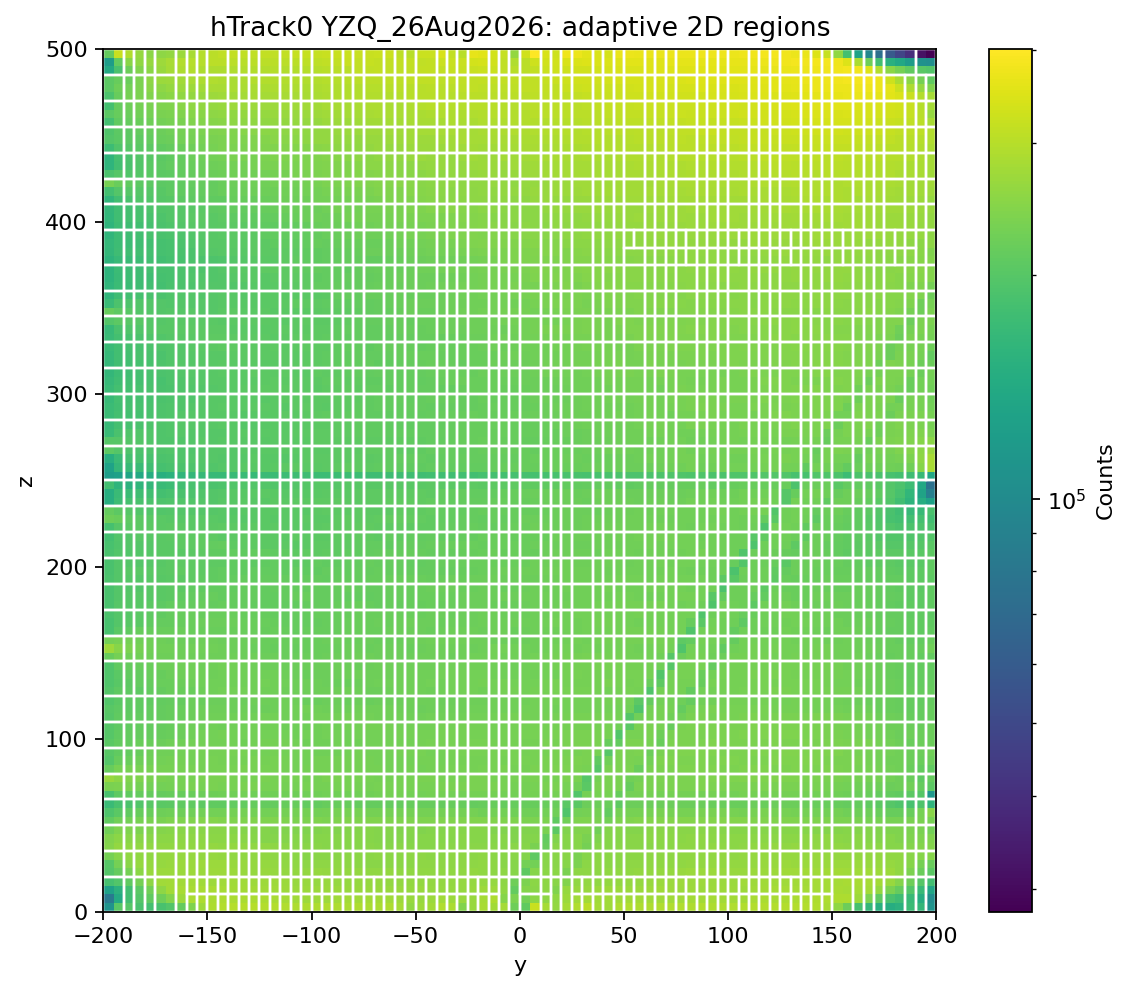
\includegraphics[width=\textwidth]{Figures/WireMod2D/adaptive/hTrack0_YZQ_26Aug2026_adaptive_2d_regions.png}
    \caption{\texttt{YZQ} adaptive regions.}
\end{subfigure}
\begin{subfigure}{0.48\textwidth}
    \centering
    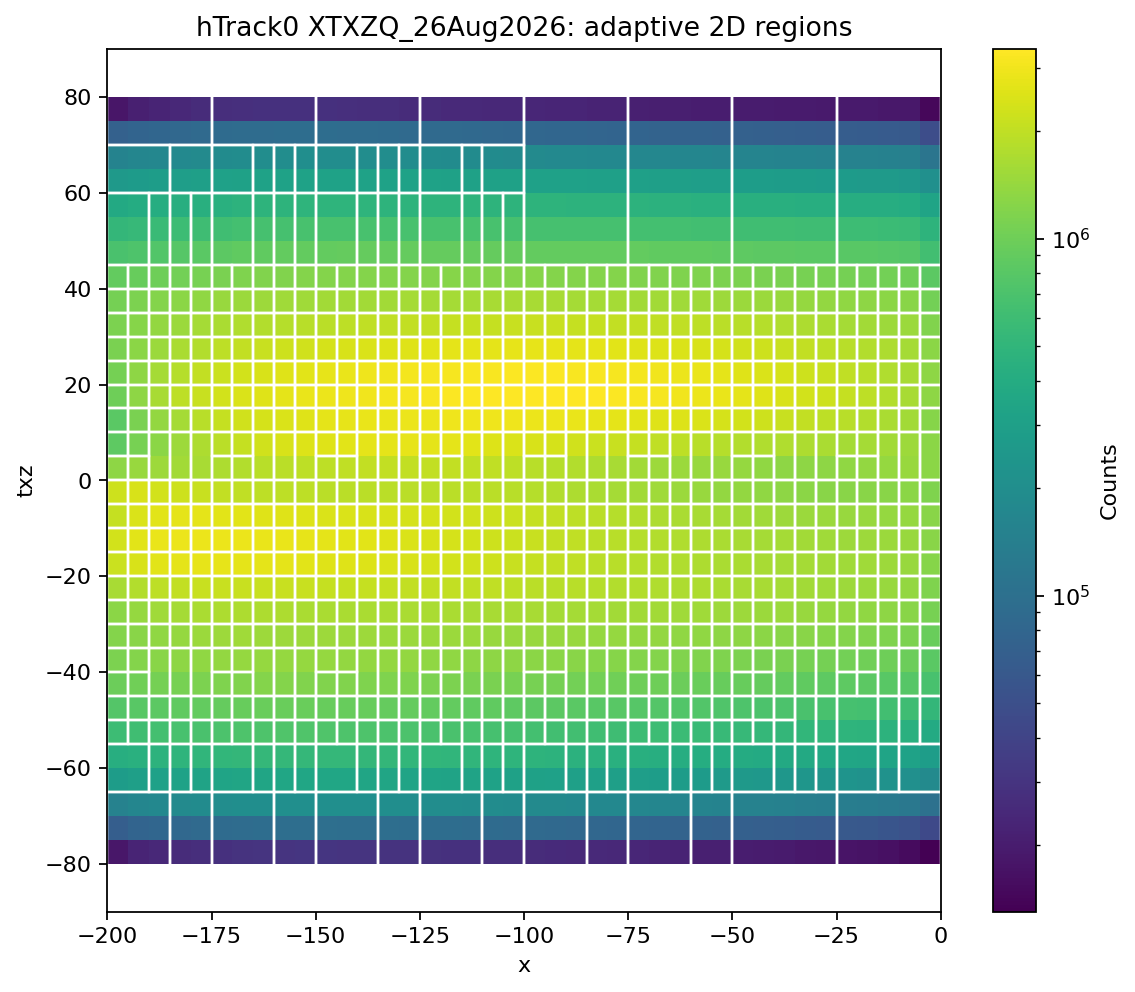
\includegraphics[width=\textwidth]{Figures/WireMod2D/adaptive/hTrack0_XTXZQ_26Aug2026_adaptive_2d_regions.png}
    \caption{\texttt{XTXZQ} adaptive regions.}
\end{subfigure}
\caption{Example adaptive 2D binnings for plane 0. The \texttt{XTXZQ} binning uses the active $x<0$ side for plane 0.}
\label{fig:wiremod_2d_adaptive_examples}
\end{figure}

\begin{figure}[H]
\centering
\begin{subfigure}{0.48\textwidth}
    \centering
    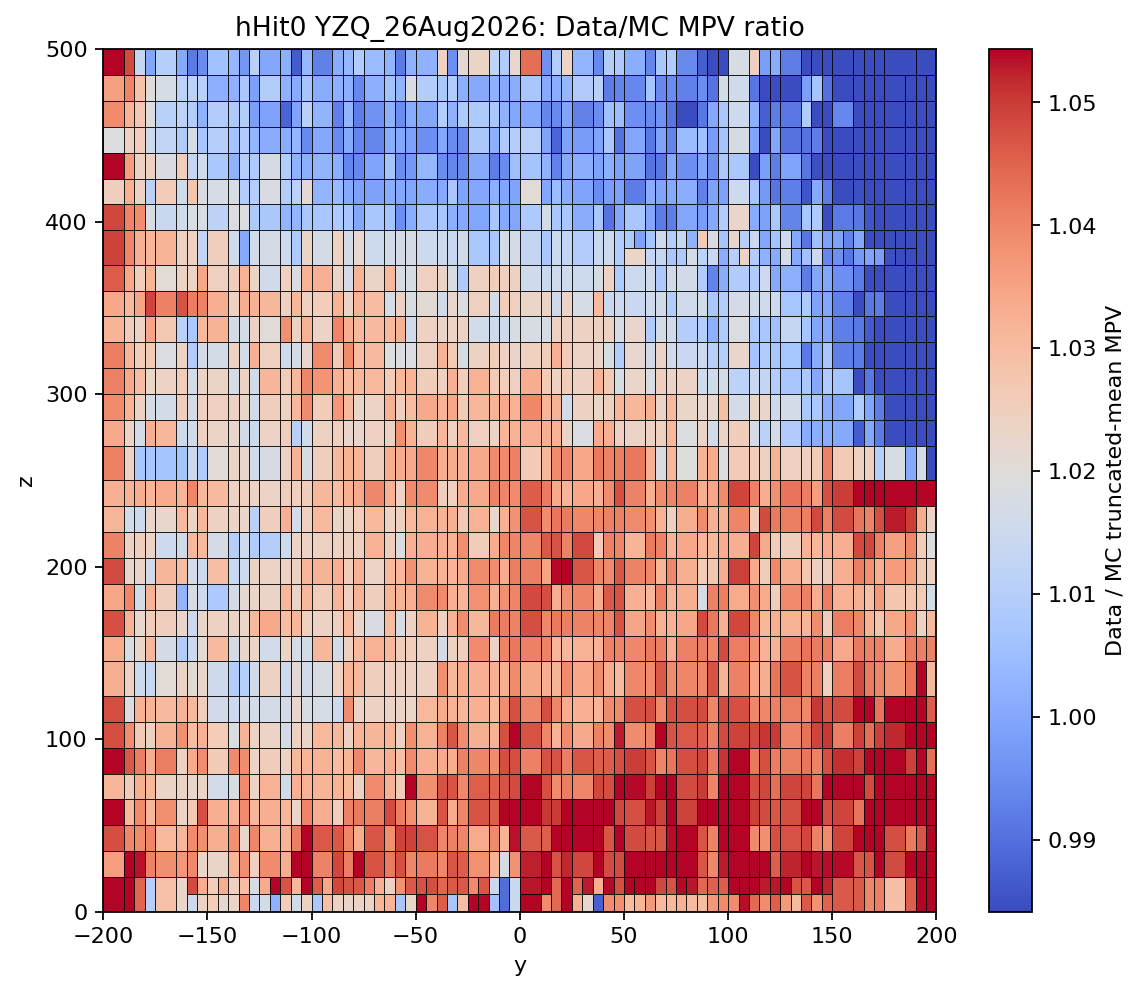
\includegraphics[width=\textwidth]{Figures/WireMod2D/ratios/YZQ_26Aug2026/hHit0_ratio_map.png}
    \caption{\texttt{YZQ} ratio map.}
\end{subfigure}
\begin{subfigure}{0.48\textwidth}
    \centering
    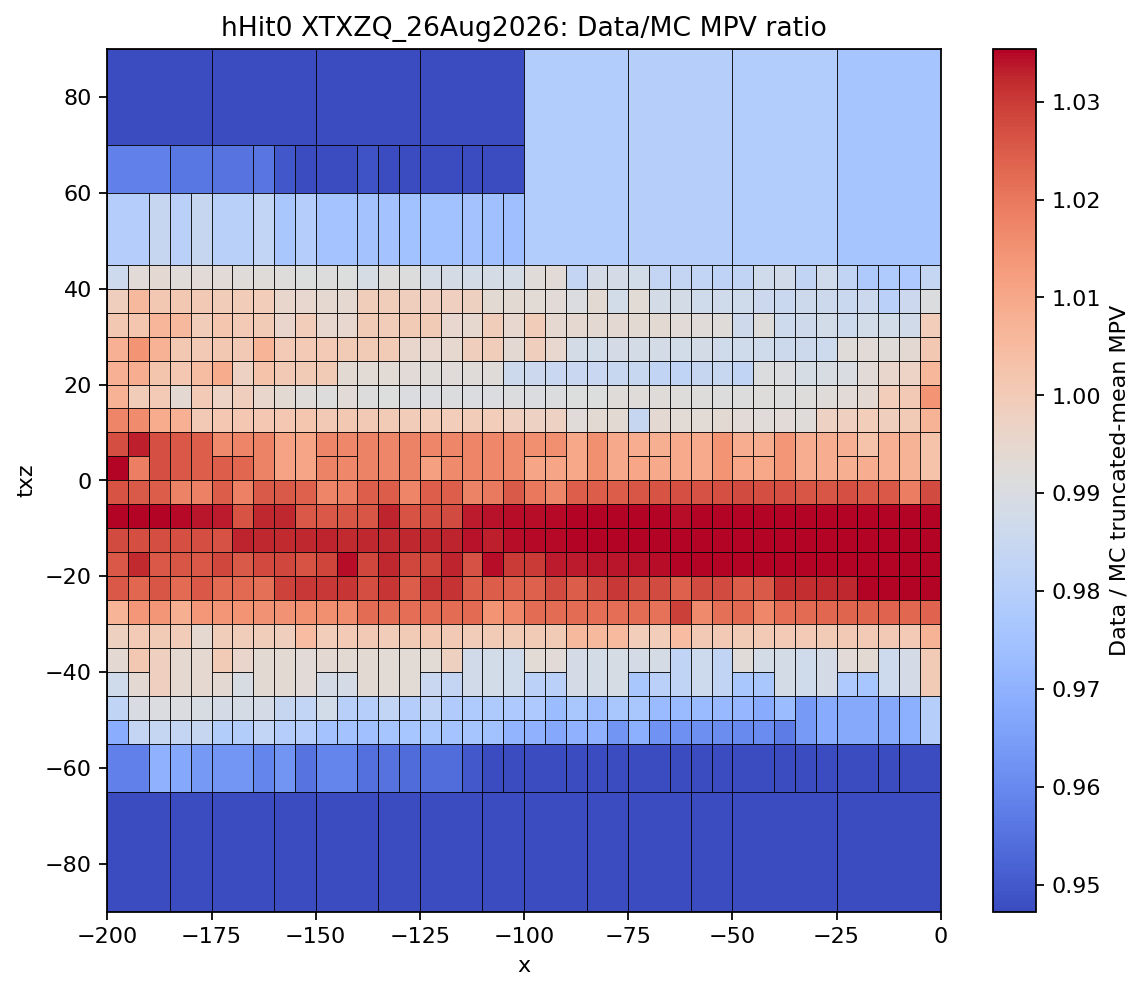
\includegraphics[width=\textwidth]{Figures/WireMod2D/ratios/XTXZQ_26Aug2026/hHit0_ratio_map.png}
    \caption{\texttt{XTXZQ} ratio map.}
\end{subfigure}
\caption{Example data/MC truncated-mean MPV ratio maps for plane 0.}
\label{fig:wiremod_2d_ratio_examples}
\end{figure}

\section{Higher Dimensional Angle-Binned Spline Generation}

\subsection{Workflow}

The higher-dimensional workflow keeps the angular dependence by first partitioning the two-dimensional angular plane, then producing separate $(x,y,z,\mathrm{response})$ histograms for each angular region. Within a fixed plane and angular region, the workflow proceeds as:
\begin{enumerate}
    \item Select a folded 2D angular bin in $(|\theta_{xw}|,|\theta_{yz}|)$.
    \item Generate data and MC \texttt{hTrackN}/\texttt{hHitN} histograms in \texttt{SBNDWireModHists} using the matching angle-bin config.
    \item Use the data \texttt{hTrackN} histogram to define adaptive YZ regions independently in each x-bin.
    \item In each x-bin and YZ region, project the data and MC \texttt{hHitN} histograms onto the response axis.
    \item Extract the data and MC truncated-mean MPVs and store the data/MC ratio as a 2D spline in the YZ plane.
\end{enumerate}

The final product for one plane and one angular bin is therefore a family of 2D YZ ratio splines, one spline for each populated x-slice. The full WireMod correction can then be viewed as a set of 2D YZ surfaces indexed by plane, angular bin, x-bin, and response observable.

\subsection{Angular Binning}

The current angular binning uses folded absolute angles, motivated by the approximate symmetry of the hit-response behavior about $\theta=0$ for both angular variables. The folded angular plane covers:
\begin{equation}
    0 \leq |\theta_{xw}| \leq 90^\circ,
    \qquad
    0 \leq |\theta_{yz}| \leq 90^\circ.
\end{equation}
The binning algorithm first separates the angular space into low-low, low-high, high-low, and high-high regions, with the high-angle boundary at approximately $60^\circ$. Adaptive splitting is then run within these regions so that high-angle regions, where stronger gradients are expected, are not swallowed by very large low-angle bins. The current target used for this angular binning is $10^{5}$ tracks per angular region.

\subsection{Adaptive YZ Binning in X Slices}

The x/YZ adaptive binning is produced with:
\begin{verbatim}
scripts/make_adaptive_binning_xyz.py
\end{verbatim}
This script expects the reduced four-dimensional sparse output from \texttt{SBNDWireModHists}, with axes corresponding to $(x,y,z,\mathrm{response})$. For each physical x-bin, it projects the data \texttt{hTrackN} histogram onto the YZ plane. If the x-bin has enough tracks, the YZ plane is adaptively split with the same quadrant-first logic used by the simple 2D workflow.

A representative command is:
\begin{verbatim}
DATA=AngleData/data/plane0
./scripts/run_with_root.sh scripts/make_adaptive_binning_xyz.py \
  --input $DATA/gen2_data_config_xyz_spline_anglebin_q_plane0_region001_full.root \
  --hist hTrack0 \
  --target 100000 \
  --max-plots 5
\end{verbatim}

The output label is inferred from names such as \texttt{anglebin\_q\_plane0\_region001}, so each angular-region binning is kept separate. The output files are written to:
\begin{verbatim}
plots/adaptive_xyz
\end{verbatim}

\subsection{XYZ Ratio Spline Extraction}

The higher-dimensional ratio extraction is performed with:
\begin{verbatim}
scripts/make_xyz_ratio_splines.py
\end{verbatim}
For each x-bin and adaptive YZ region, the script projects the data and MC \texttt{hHitN} histograms onto the response axis and applies the same iterative truncated-mean MPV extraction used in the simple 2D workflow. The output ROOT file contains one set of graphs per x-bin:
\begin{itemize}
    \item \texttt{data\_mpv\_N\_X}: data MPV graph in the YZ plane,
    \item \texttt{mc\_mpv\_N\_X}: MC MPV graph in the YZ plane,
    \item \texttt{splines\_N\_X}: data/MC ratio graph in the YZ plane.
\end{itemize}
Here $N$ is the plane index and $X$ is the x-bin index.

A representative command for charge is:
\begin{verbatim}
DATA=AngleData/data/plane0
MC=AngleData/mc/plane0
./scripts/run_with_root.sh scripts/make_xyz_ratio_splines.py \
  --data $DATA/gen2_data_config_xyz_spline_anglebin_q_plane0_region001_full.root \
  --mc $MC/gen2_mc_config_xyz_spline_anglebin_q_plane0_region001_full.root \
  --hit-hist hHit0 \
  --idx 0
\end{verbatim}

For \texttt{dq} or \texttt{w}, the same charge-derived adaptive YZ binning can be reused with:
\begin{verbatim}
--binning-observable q
\end{verbatim}
This keeps the spatial binning fixed across response observables for the same plane and angular region.

\subsection{Current Higher-Dimensional Tests}

The current end-to-end higher-dimensional test has been run for plane 0, angular region 001, and the \texttt{q}, \texttt{dq}, and \texttt{w} observables. Diagnostic outputs include adaptive YZ region plots for individual x-bins, YZ ratio maps for each x-bin, and optional per-region hit-response plots with data and MC MPV markers.

\Cref{fig:wiremod_xyz_adaptive_example,fig:wiremod_xyz_ratio_example} show representative plane-0, region-001 outputs. These are useful debugging plots for checking that the YZ binning follows the data track density and that the extracted ratios vary smoothly within each x-slice.

\begin{figure}[H]
\centering
\begin{subfigure}{0.24\textwidth}
    \centering
    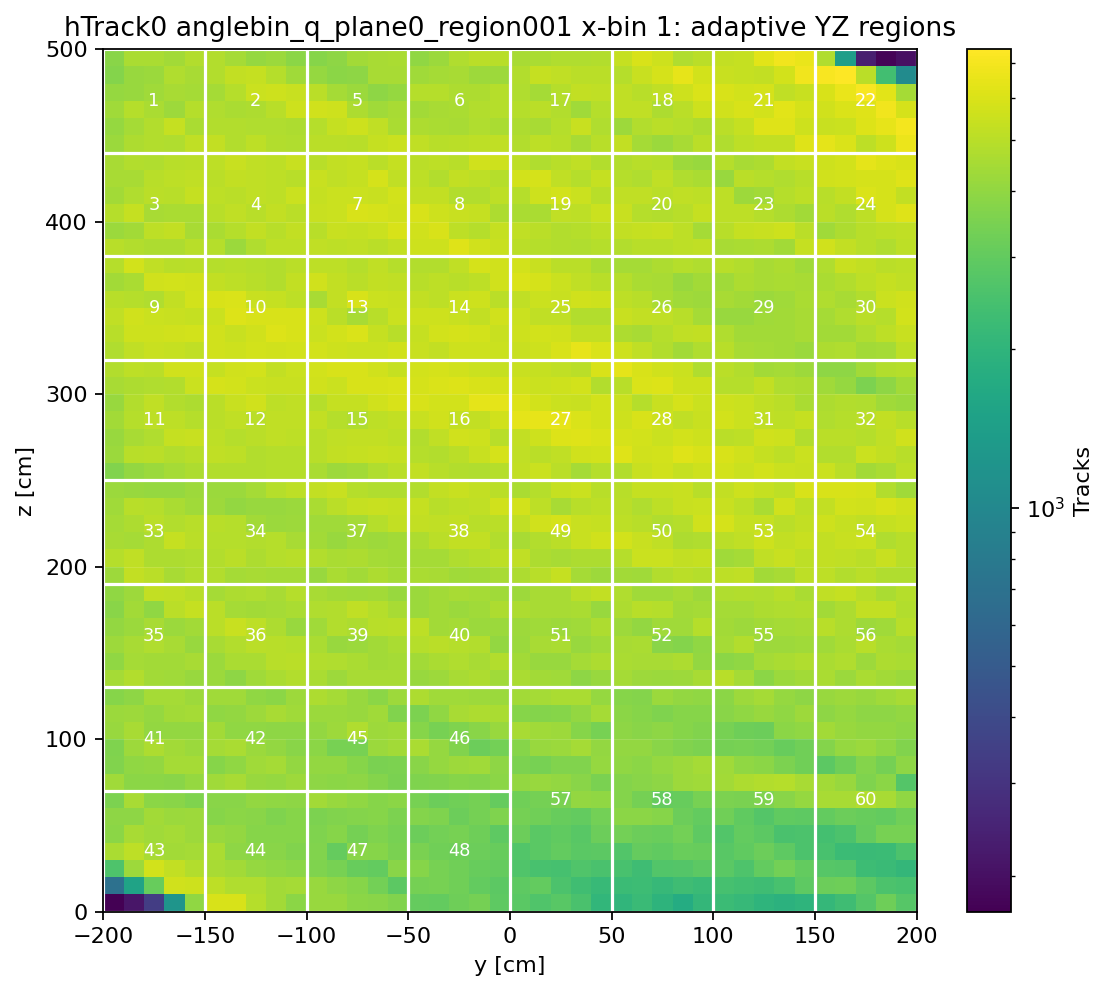
\includegraphics[width=\textwidth]{Figures/WireModXYZ/adaptive/hTrack0_anglebin_q_plane0_region001_adaptive_yz_regions_by_x_xbin001_adaptive_yz.png}
    \caption{x-bin 1}
\end{subfigure}
\begin{subfigure}{0.24\textwidth}
    \centering
    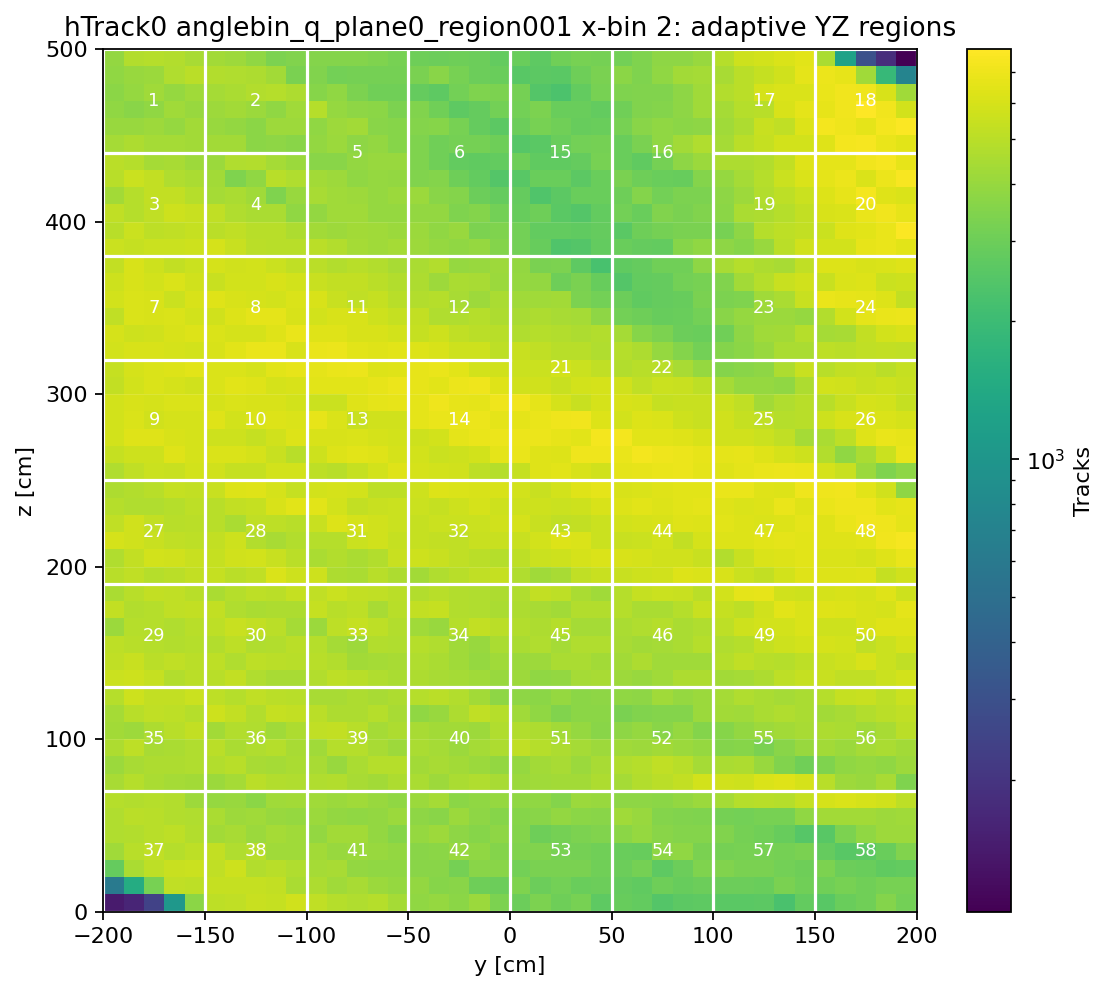
\includegraphics[width=\textwidth]{Figures/WireModXYZ/adaptive/hTrack0_anglebin_q_plane0_region001_adaptive_yz_regions_by_x_xbin002_adaptive_yz.png}
    \caption{x-bin 2}
\end{subfigure}
\begin{subfigure}{0.24\textwidth}
    \centering
    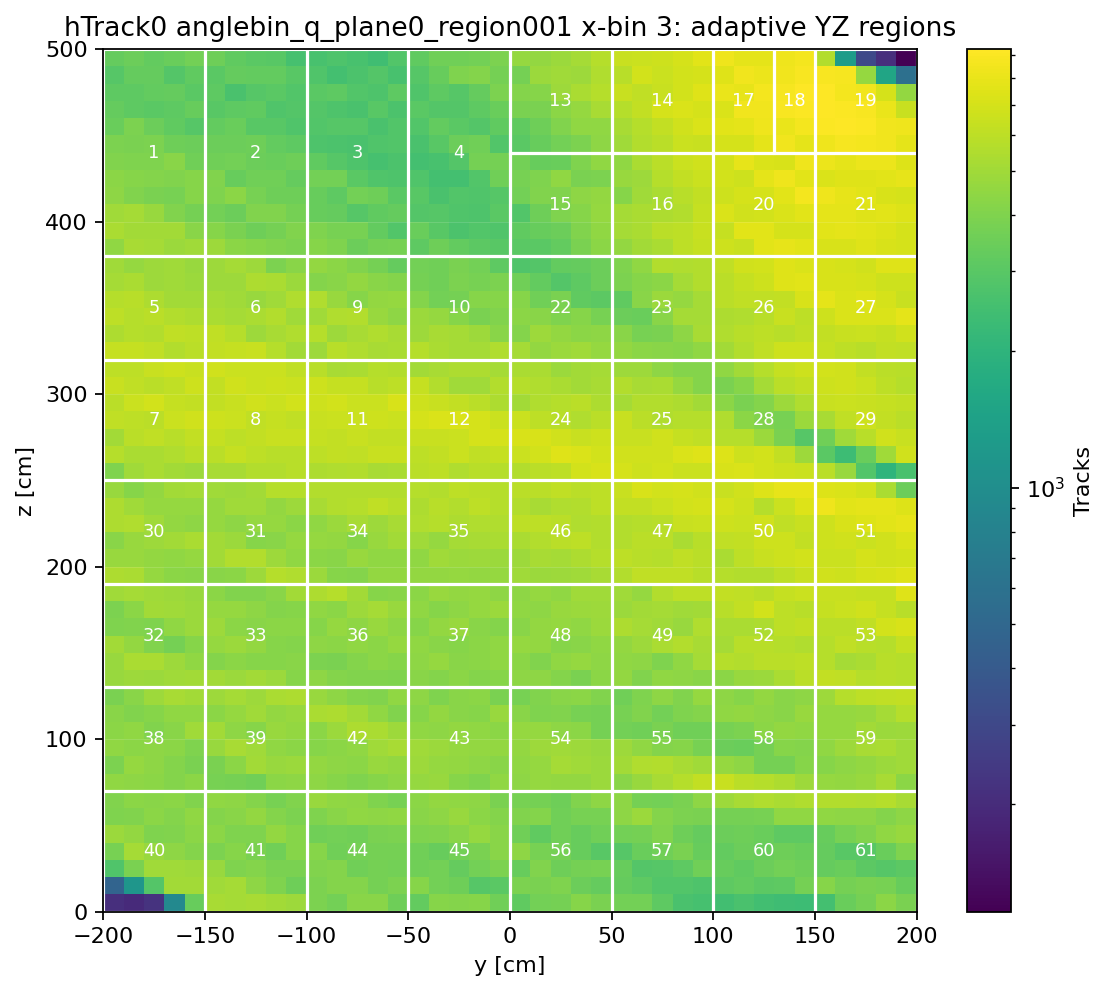
\includegraphics[width=\textwidth]{Figures/WireModXYZ/adaptive/hTrack0_anglebin_q_plane0_region001_adaptive_yz_regions_by_x_xbin003_adaptive_yz.png}
    \caption{x-bin 3}
\end{subfigure}
\begin{subfigure}{0.24\textwidth}
    \centering
    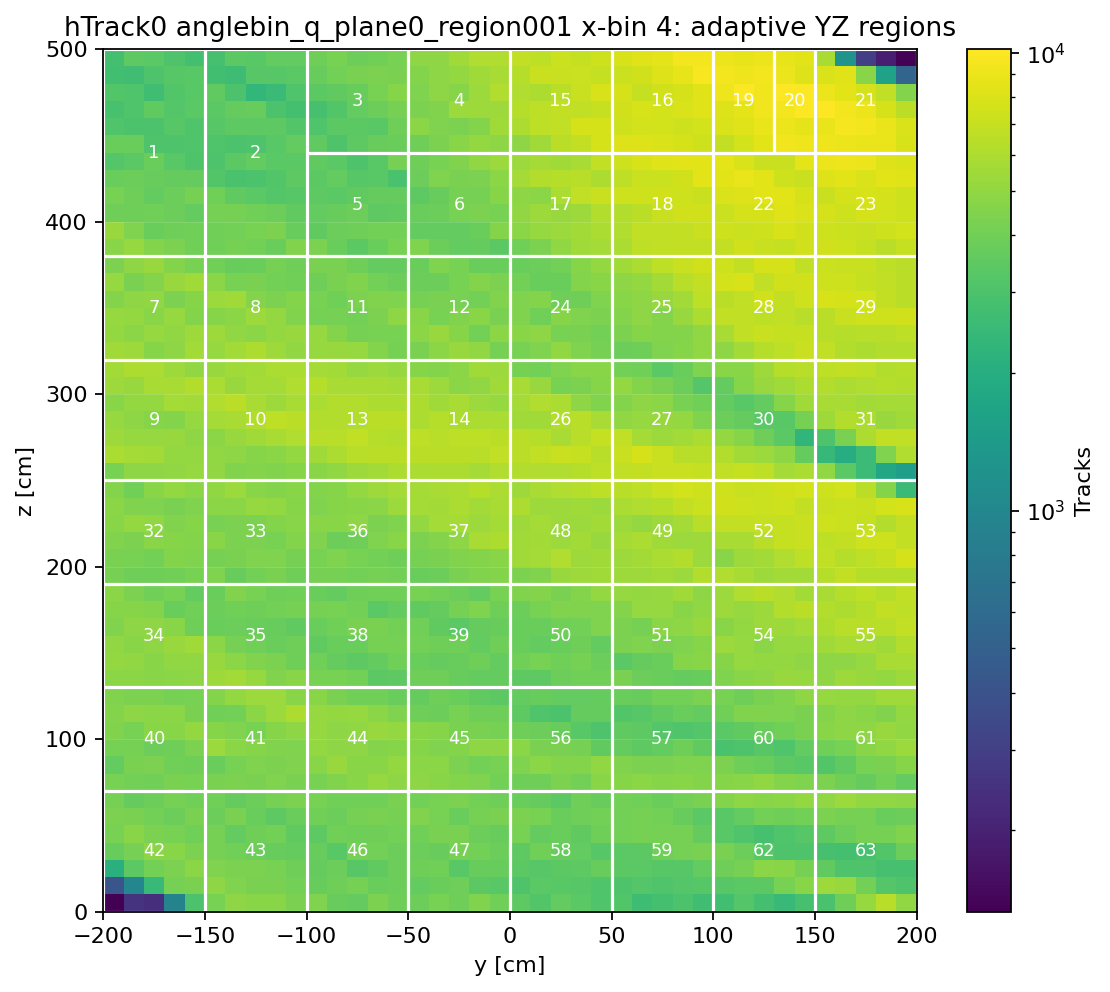
\includegraphics[width=\textwidth]{Figures/WireModXYZ/adaptive/hTrack0_anglebin_q_plane0_region001_adaptive_yz_regions_by_x_xbin004_adaptive_yz.png}
    \caption{x-bin 4}
\end{subfigure}
\caption{Example adaptive YZ regions for plane 0, angular region 001, in the first four x-bins.}
\label{fig:wiremod_xyz_adaptive_example}
\end{figure}

\begin{figure}[H]
\centering
\begin{subfigure}{0.31\textwidth}
    \centering
    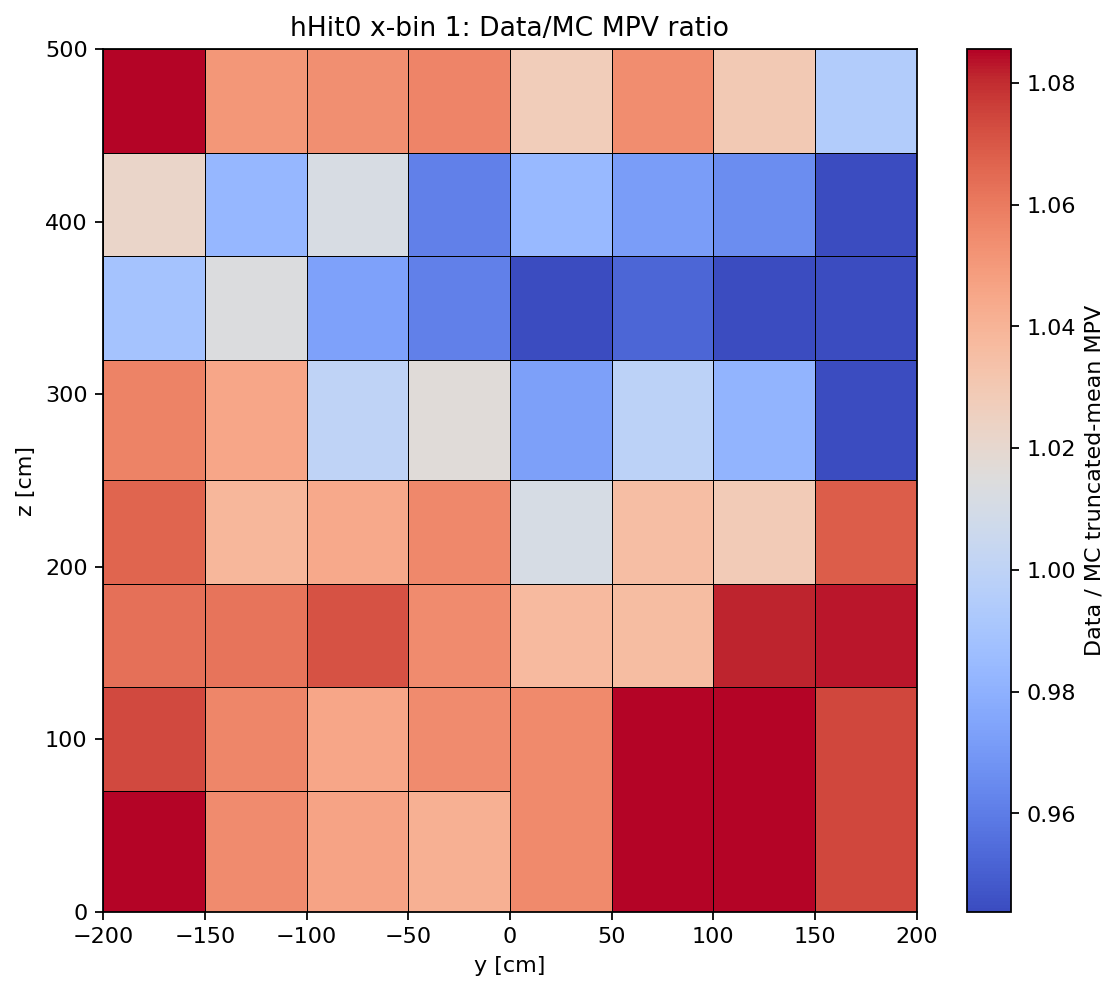
\includegraphics[width=\textwidth]{Figures/WireModXYZ/ratios/q/hHit0_xbin001_ratio_map.png}
    \caption{$Q$, x-bin 1}
\end{subfigure}
\begin{subfigure}{0.31\textwidth}
    \centering
    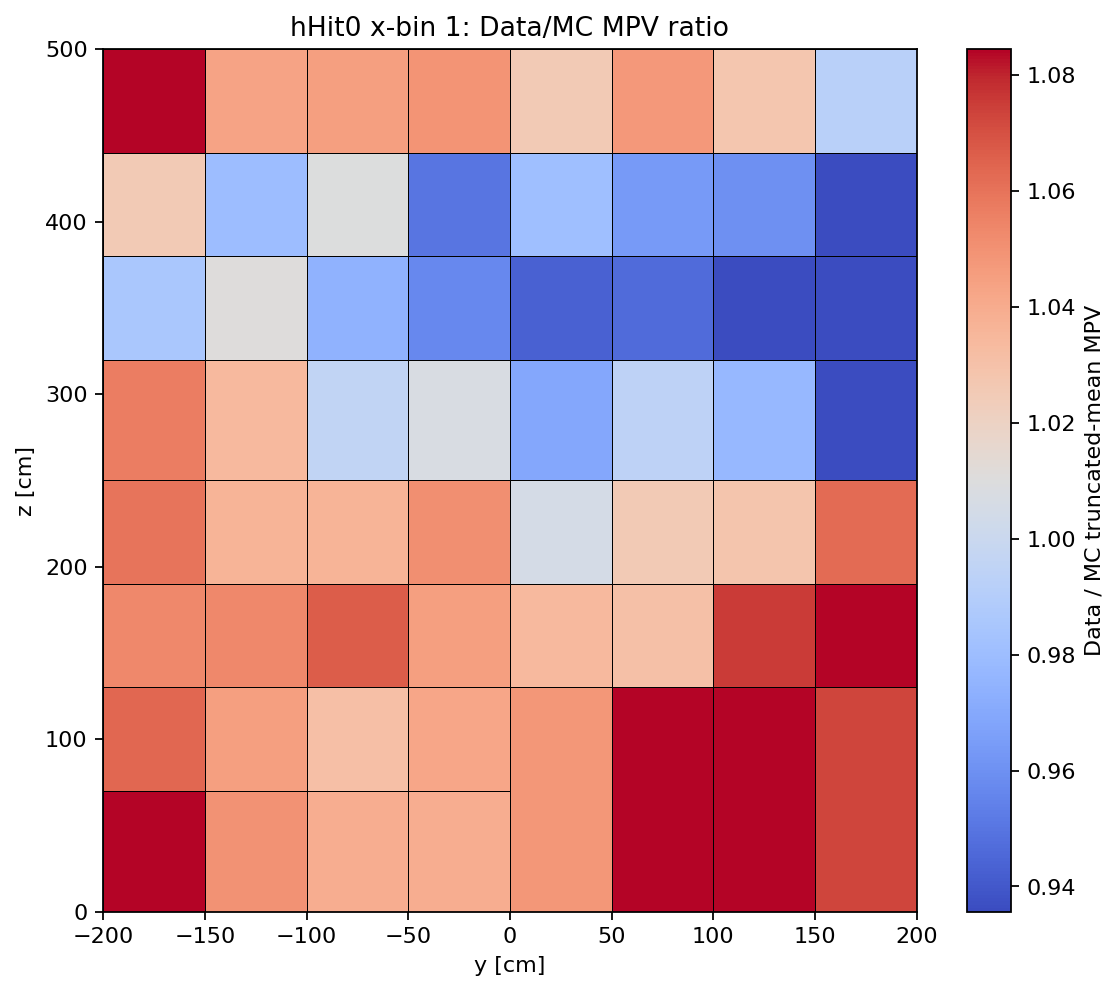
\includegraphics[width=\textwidth]{Figures/WireModXYZ/ratios/dq/hHit0_xbin001_ratio_map.png}
    \caption{dQ/dx, x-bin 1}
\end{subfigure}
\begin{subfigure}{0.31\textwidth}
    \centering
    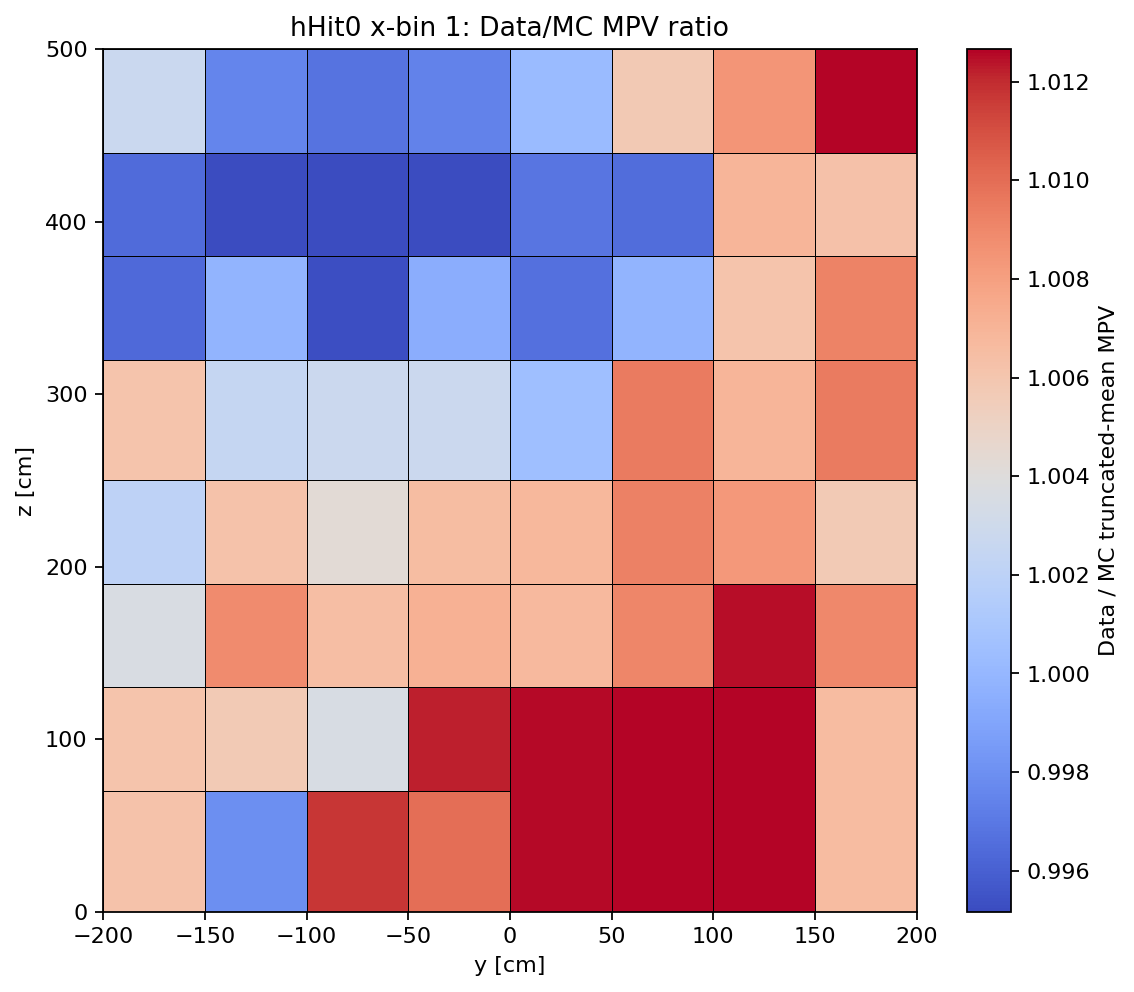
\includegraphics[width=\textwidth]{Figures/WireModXYZ/ratios/w/hHit0_xbin001_ratio_map.png}
    \caption{Width, x-bin 1}
\end{subfigure}
\caption{Example YZ data/MC MPV ratio maps for plane 0, angular region 001, and three response observables.}
\label{fig:wiremod_xyz_ratio_example}
\end{figure}



\printbibliography[heading=bibintoc,title=References]

\pagebreak

\begin{appendices}



\section{\label{sec:appendix_gen2_2d} 2D Splines in Gen2}

\subsection{Adaptive Binning Diagnostics}

\begin{figure}[H]
\centering
\begin{subfigure}{0.31\textwidth}\centering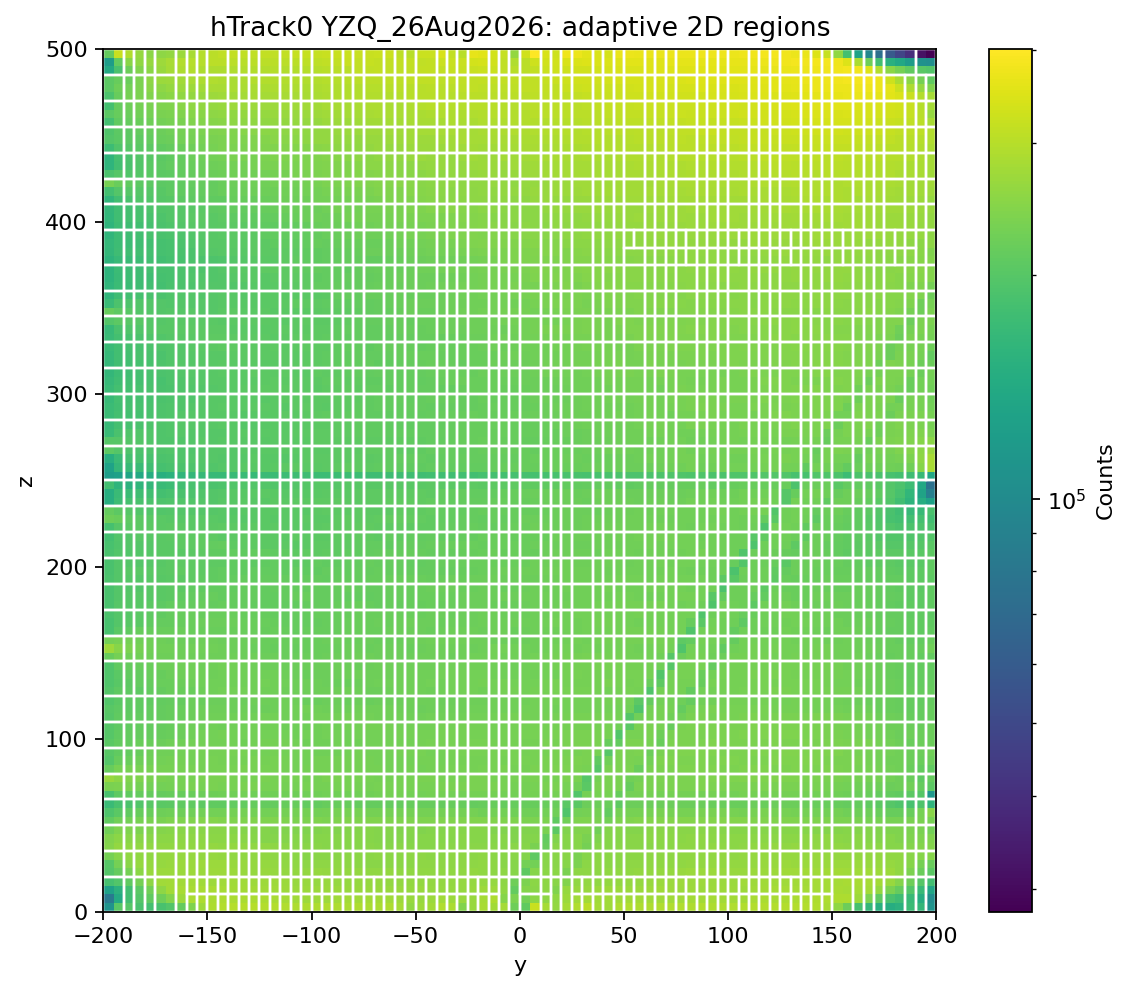
\includegraphics[width=\textwidth]{Figures/WireMod2D/adaptive/hTrack0_YZQ_26Aug2026_adaptive_2d_regions.png}\caption{Plane 0}\end{subfigure}
\begin{subfigure}{0.31\textwidth}\centering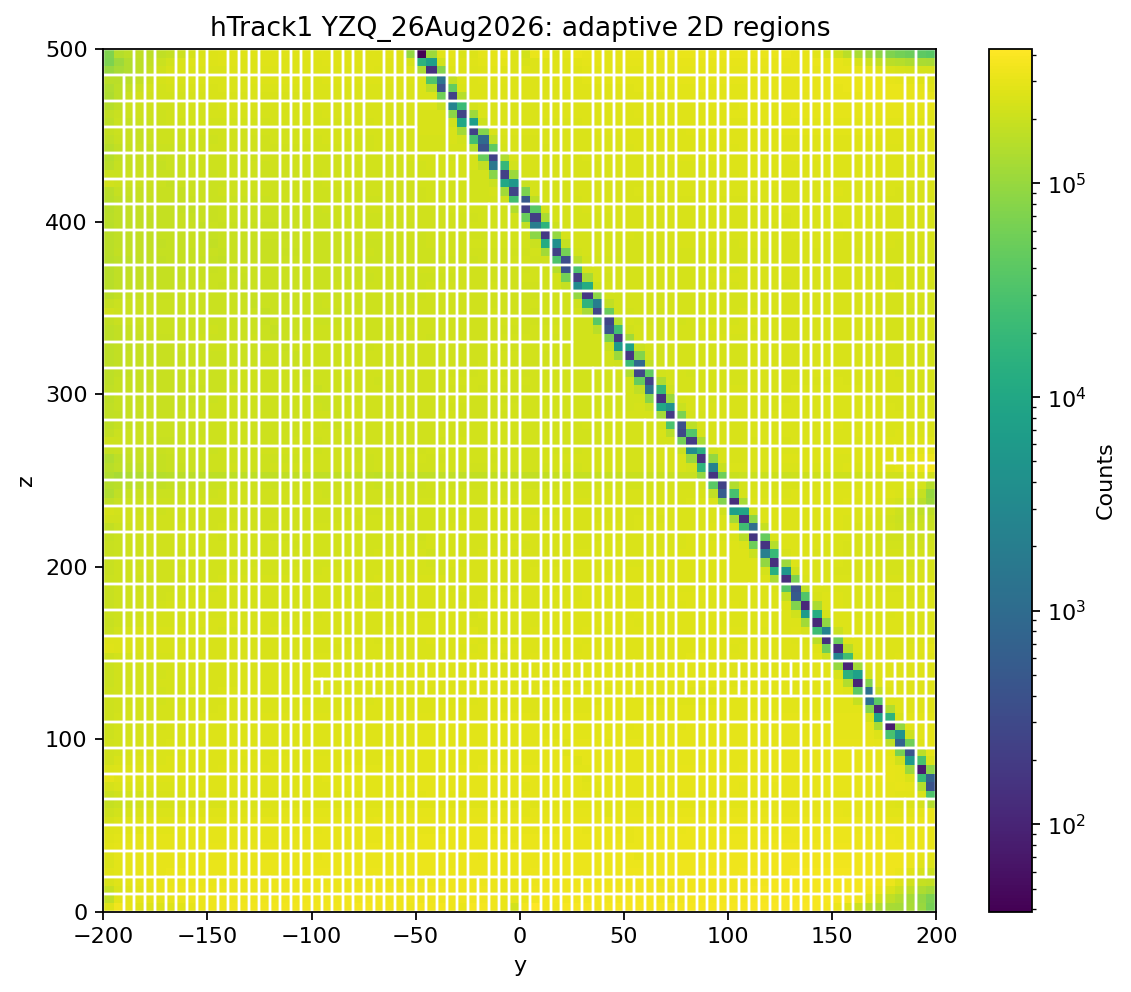
\includegraphics[width=\textwidth]{Figures/WireMod2D/adaptive/hTrack1_YZQ_26Aug2026_adaptive_2d_regions.png}\caption{Plane 1}\end{subfigure}
\begin{subfigure}{0.31\textwidth}\centering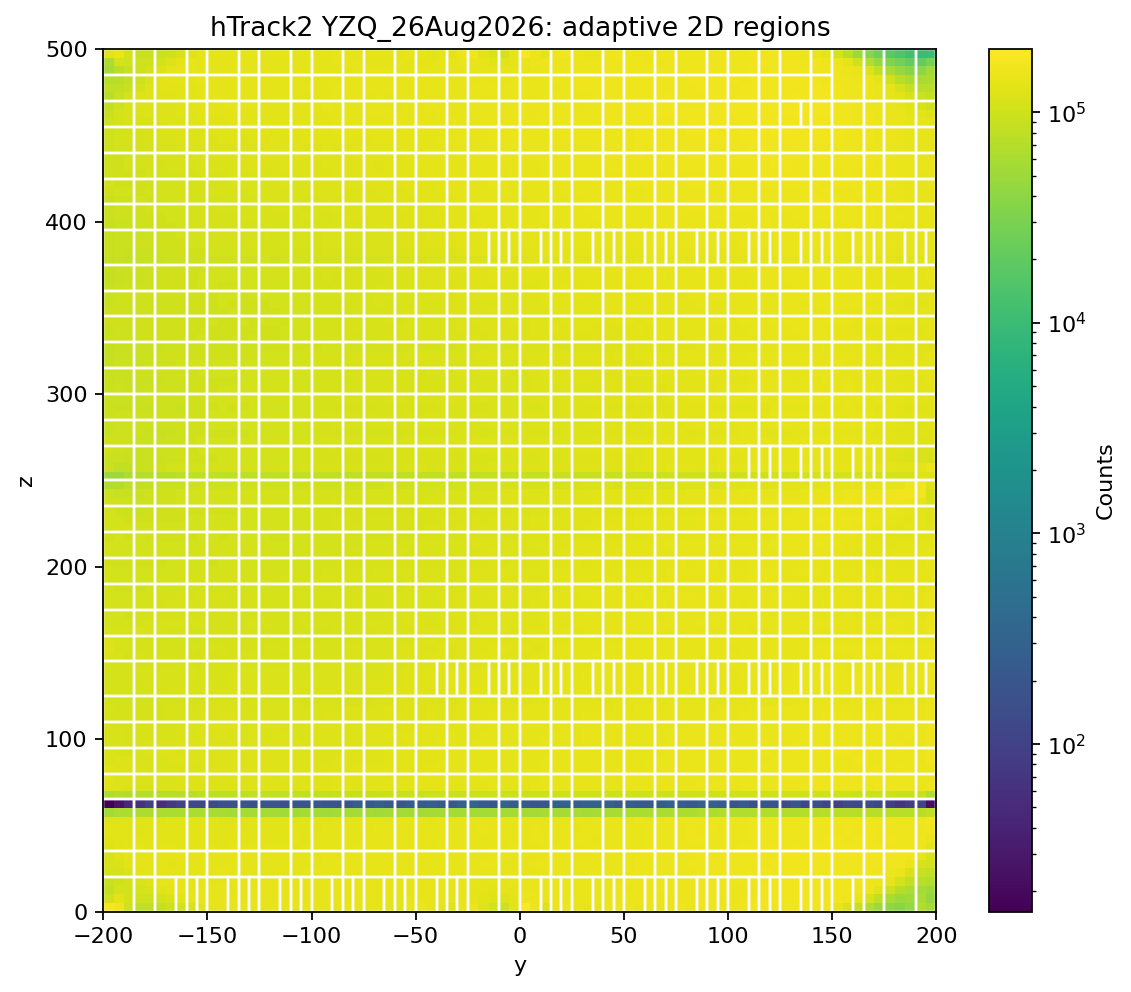
\includegraphics[width=\textwidth]{Figures/WireMod2D/adaptive/hTrack2_YZQ_26Aug2026_adaptive_2d_regions.png}\caption{Plane 2}\end{subfigure}
\begin{subfigure}{0.31\textwidth}\centering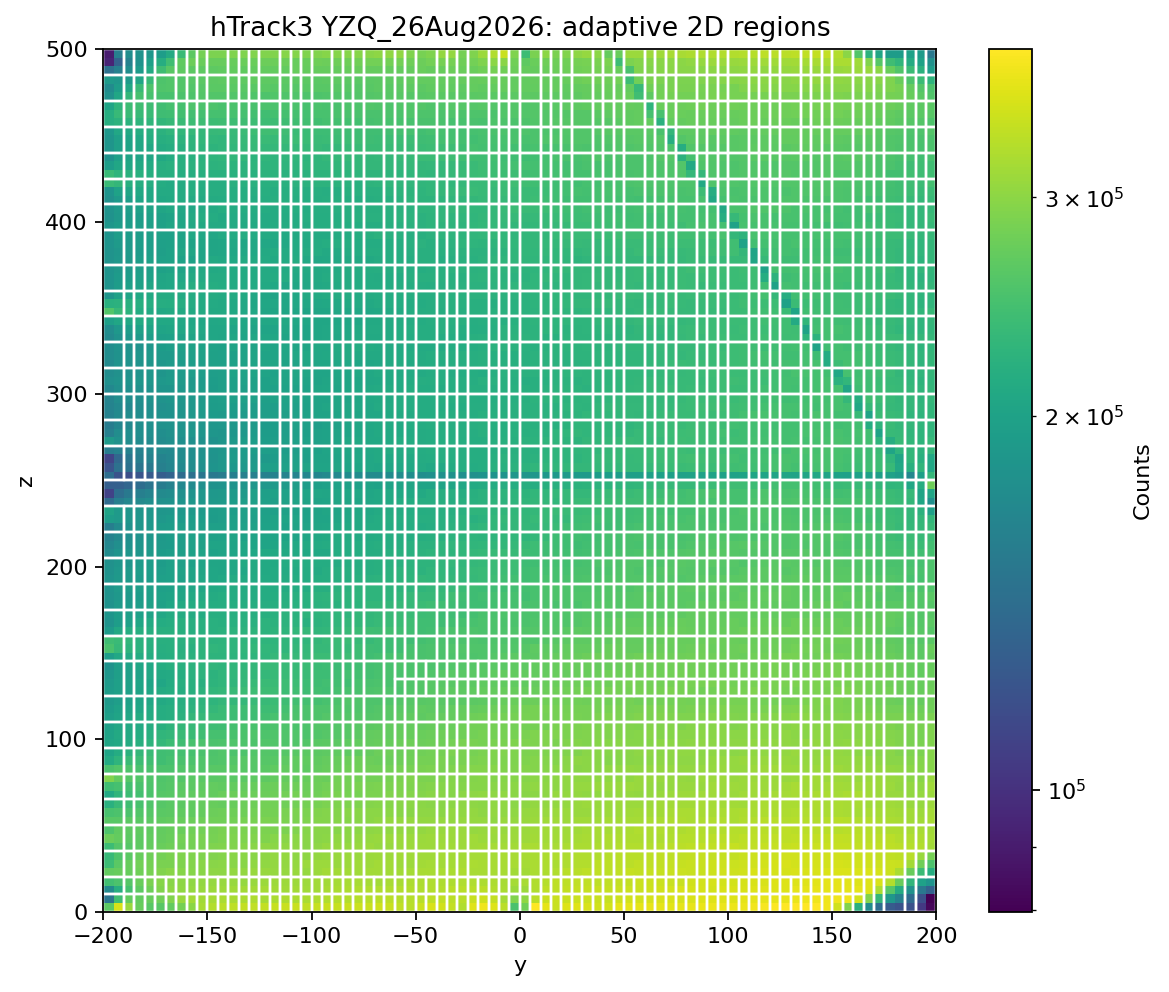
\includegraphics[width=\textwidth]{Figures/WireMod2D/adaptive/hTrack3_YZQ_26Aug2026_adaptive_2d_regions.png}\caption{Plane 3}\end{subfigure}
\begin{subfigure}{0.31\textwidth}\centering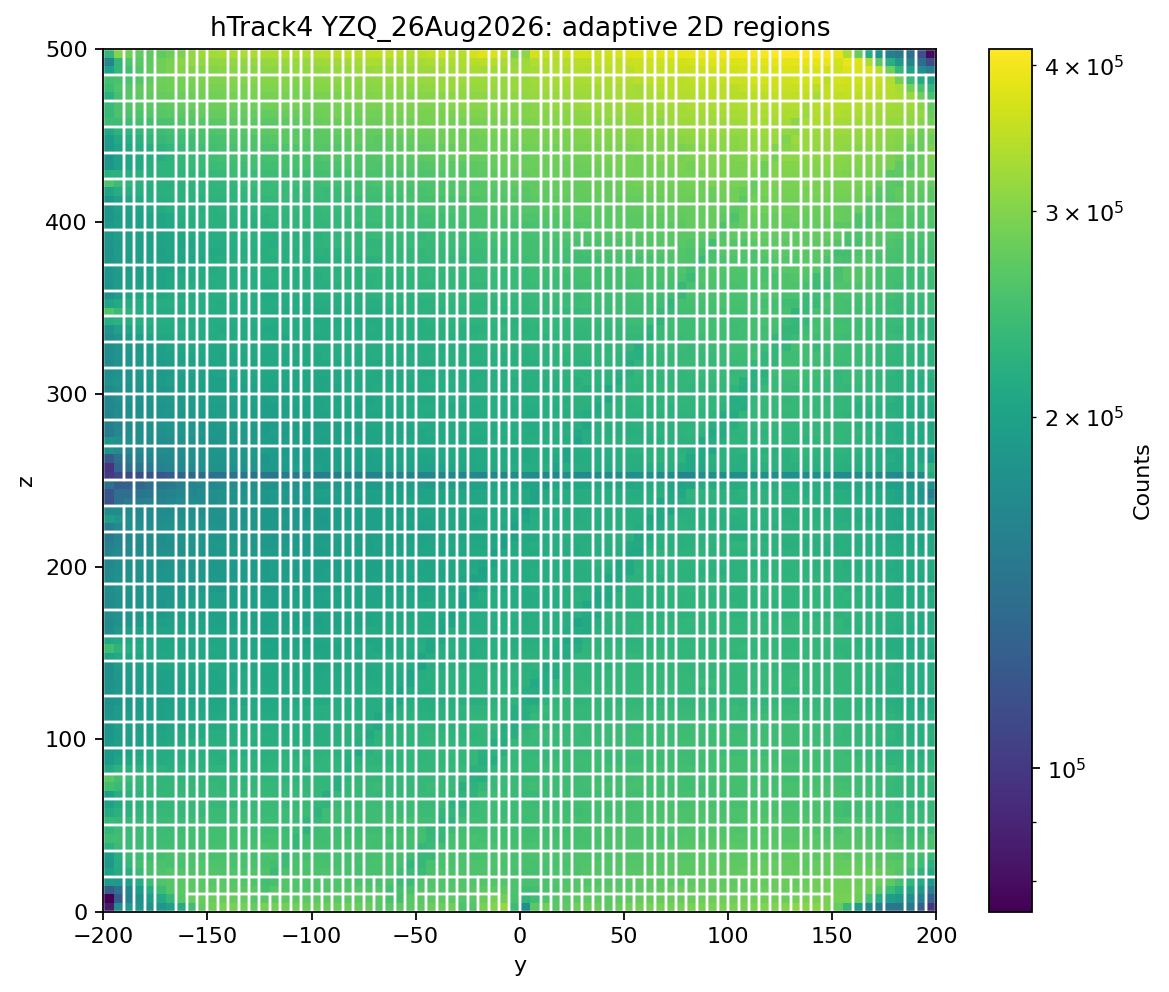
\includegraphics[width=\textwidth]{Figures/WireMod2D/adaptive/hTrack4_YZQ_26Aug2026_adaptive_2d_regions.png}\caption{Plane 4}\end{subfigure}
\begin{subfigure}{0.31\textwidth}\centering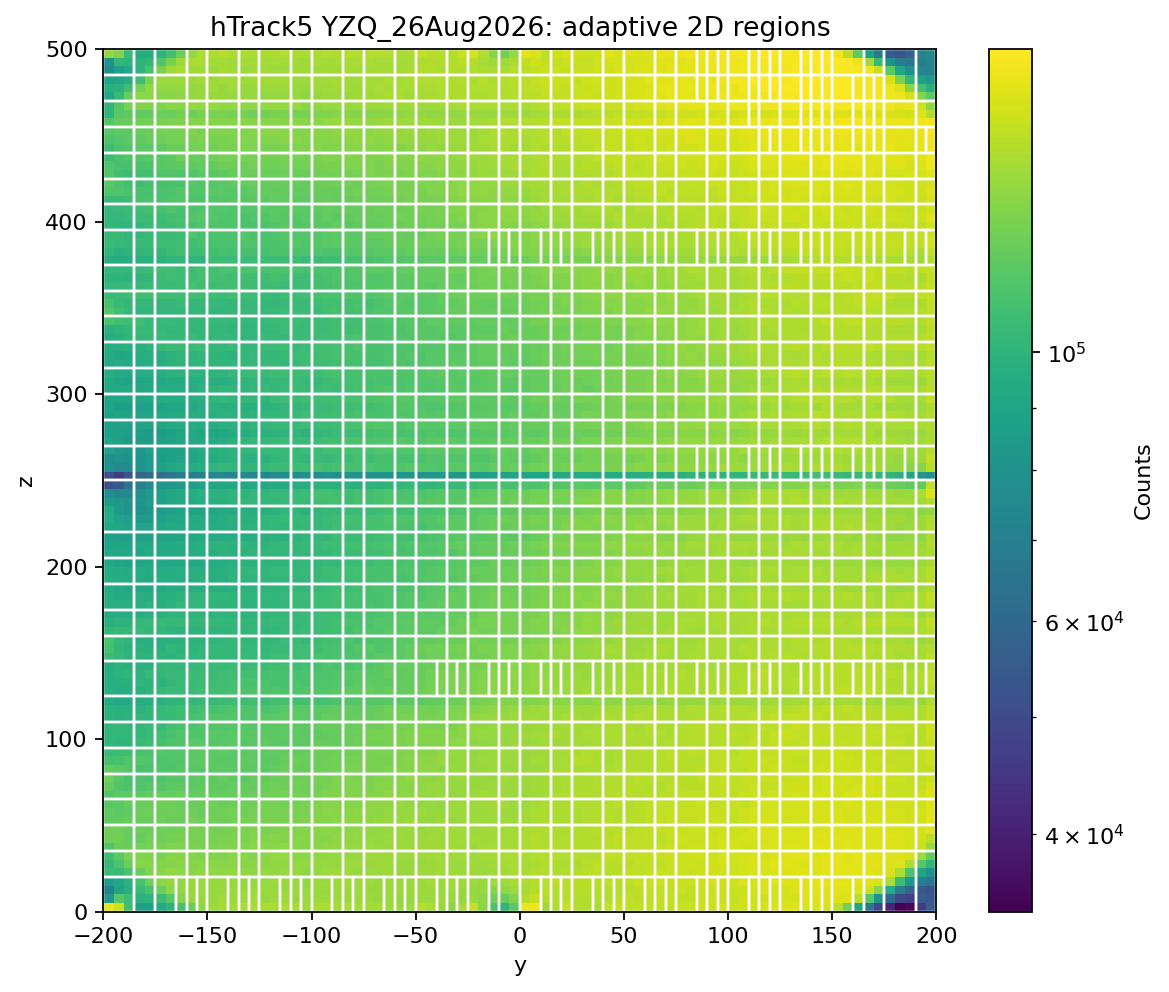
\includegraphics[width=\textwidth]{Figures/WireMod2D/adaptive/hTrack5_YZQ_26Aug2026_adaptive_2d_regions.png}\caption{Plane 5}\end{subfigure}
\caption{\texttt{YZQ} adaptive 2D regions for all planes.}
\end{figure}

\begin{figure}[H]
\centering
\begin{subfigure}{0.31\textwidth}\centering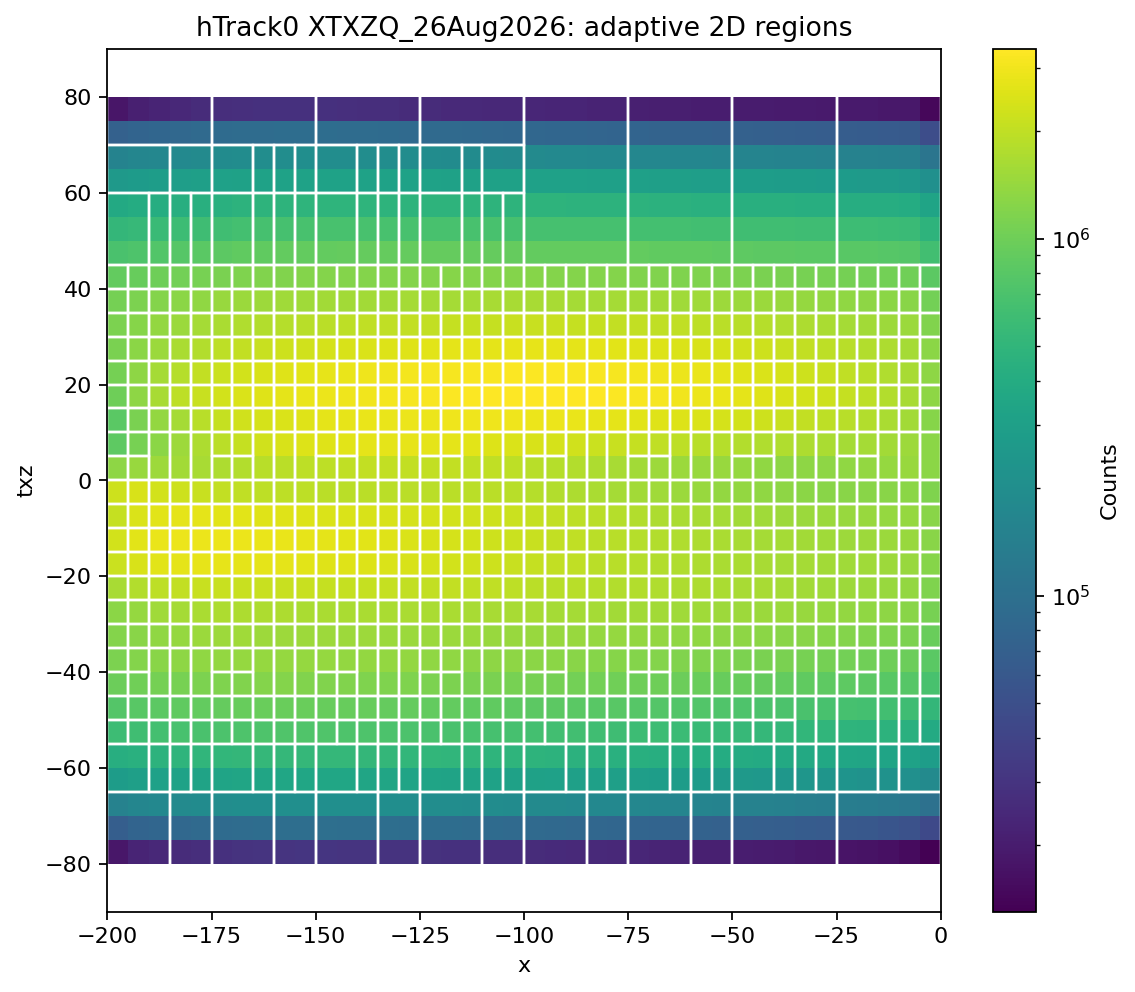
\includegraphics[width=\textwidth]{Figures/WireMod2D/adaptive/hTrack0_XTXZQ_26Aug2026_adaptive_2d_regions.png}\caption{Plane 0}\end{subfigure}
\begin{subfigure}{0.31\textwidth}\centering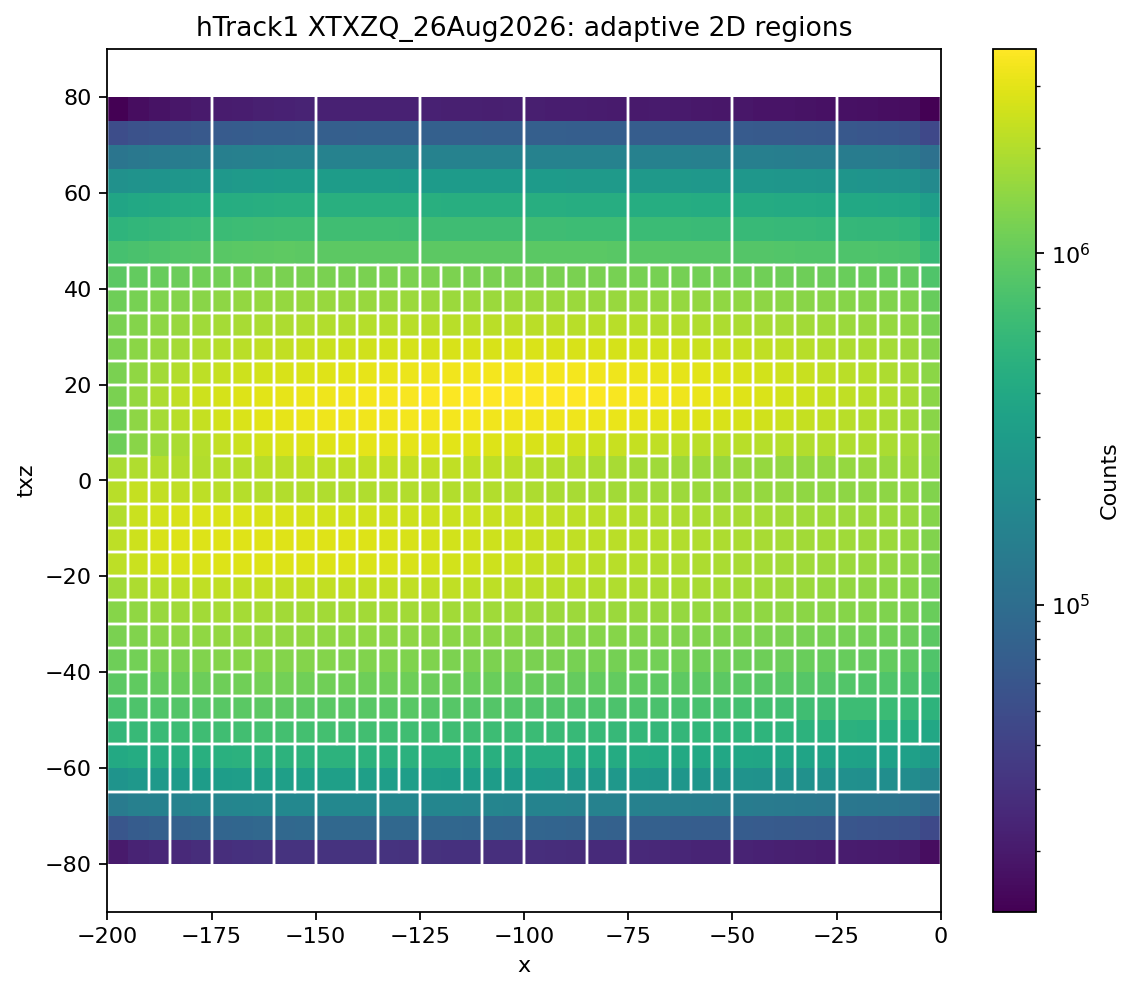
\includegraphics[width=\textwidth]{Figures/WireMod2D/adaptive/hTrack1_XTXZQ_26Aug2026_adaptive_2d_regions.png}\caption{Plane 1}\end{subfigure}
\begin{subfigure}{0.31\textwidth}\centering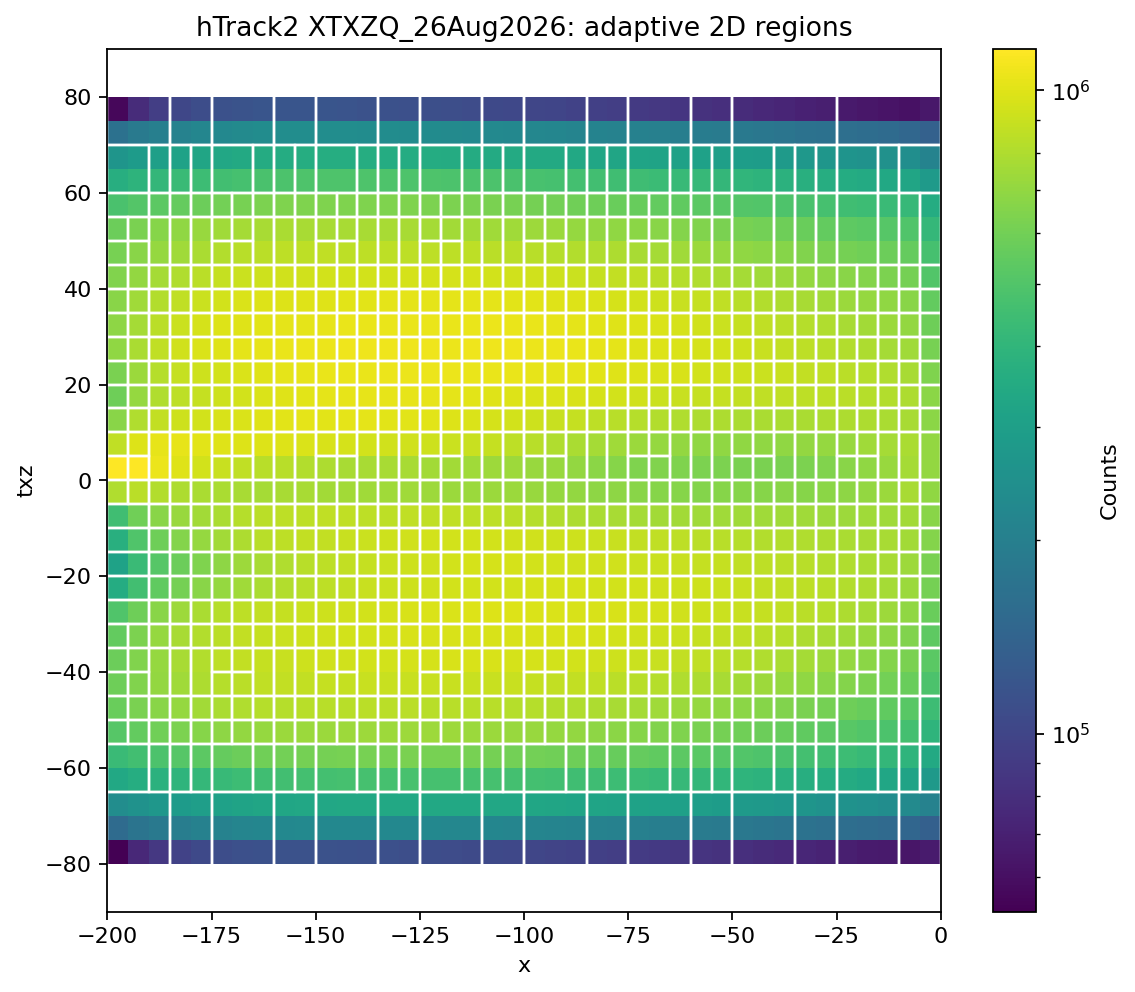
\includegraphics[width=\textwidth]{Figures/WireMod2D/adaptive/hTrack2_XTXZQ_26Aug2026_adaptive_2d_regions.png}\caption{Plane 2}\end{subfigure}
\begin{subfigure}{0.31\textwidth}\centering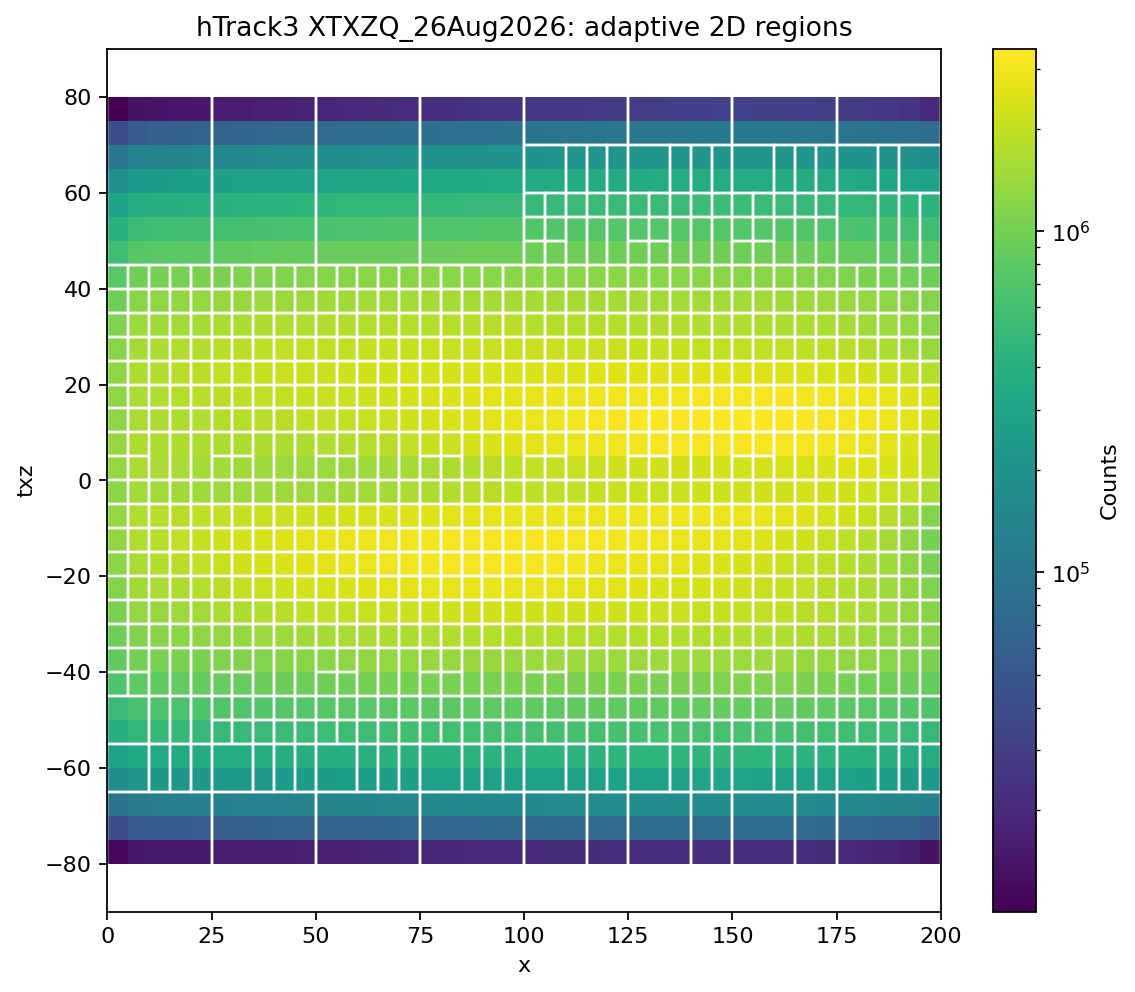
\includegraphics[width=\textwidth]{Figures/WireMod2D/adaptive/hTrack3_XTXZQ_26Aug2026_adaptive_2d_regions.png}\caption{Plane 3}\end{subfigure}
\begin{subfigure}{0.31\textwidth}\centering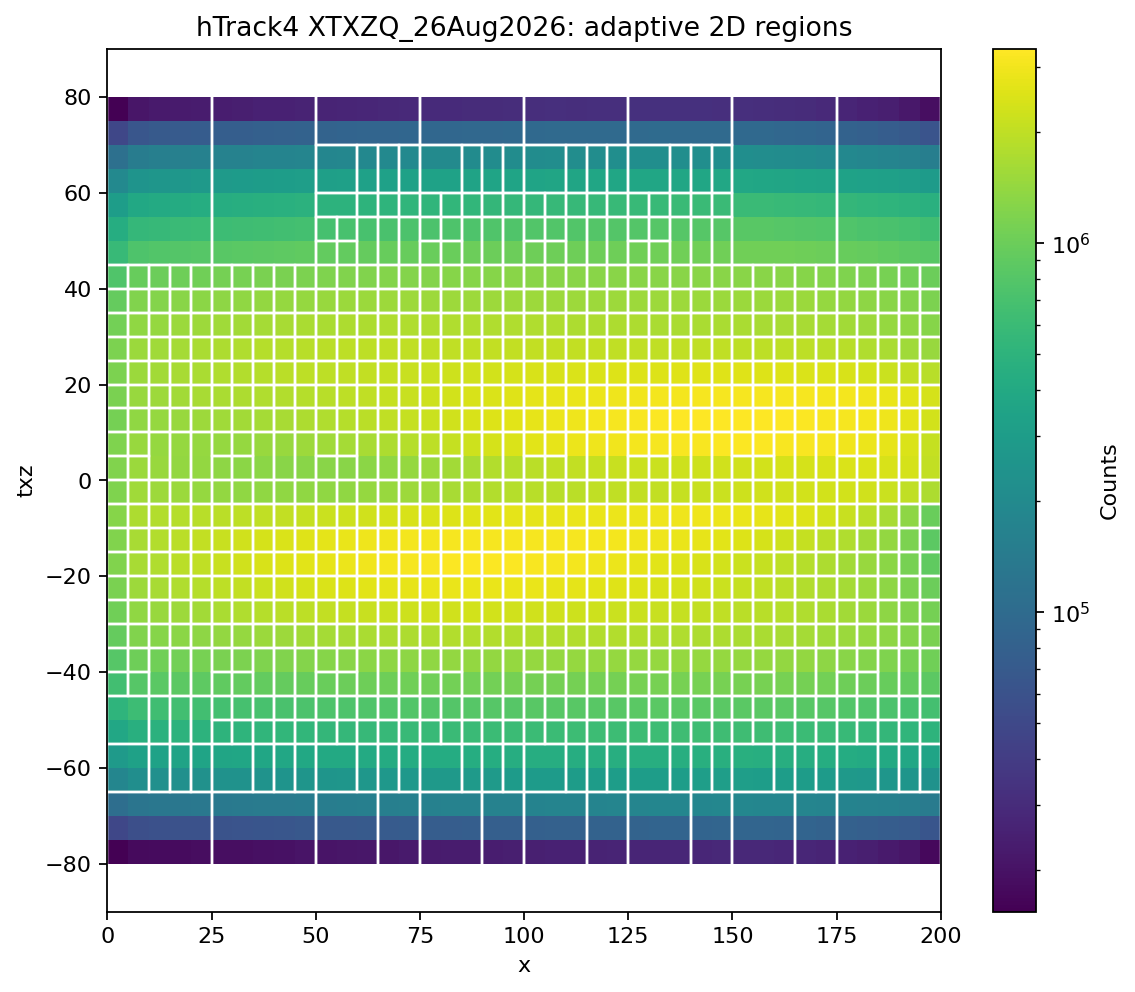
\includegraphics[width=\textwidth]{Figures/WireMod2D/adaptive/hTrack4_XTXZQ_26Aug2026_adaptive_2d_regions.png}\caption{Plane 4}\end{subfigure}
\begin{subfigure}{0.31\textwidth}\centering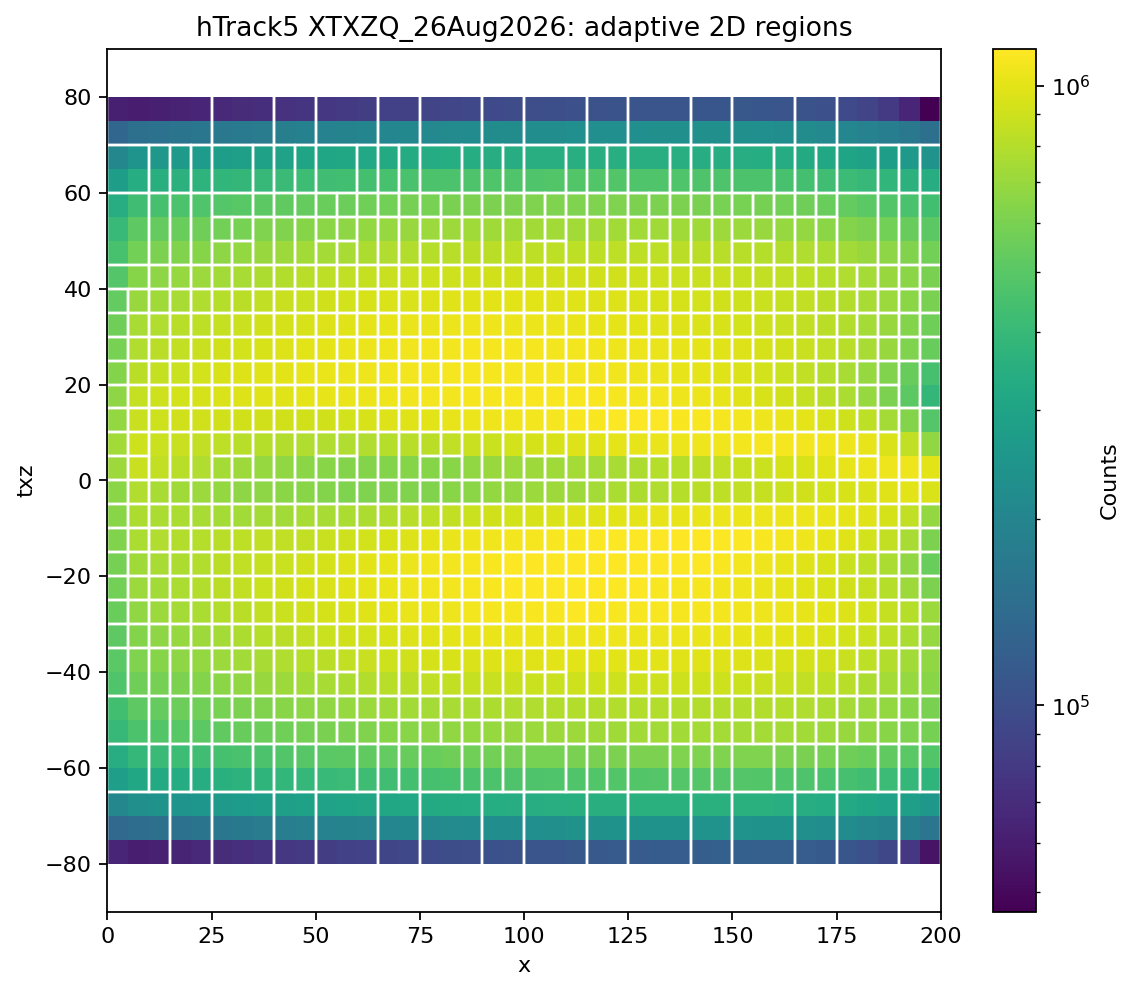
\includegraphics[width=\textwidth]{Figures/WireMod2D/adaptive/hTrack5_XTXZQ_26Aug2026_adaptive_2d_regions.png}\caption{Plane 5}\end{subfigure}
\caption{\texttt{XTXZQ} adaptive 2D regions for all planes.}
\end{figure}

\subsection{Ratio Map Diagnostics}

\begin{figure}[H]
\centering
\begin{subfigure}{0.31\textwidth}\centering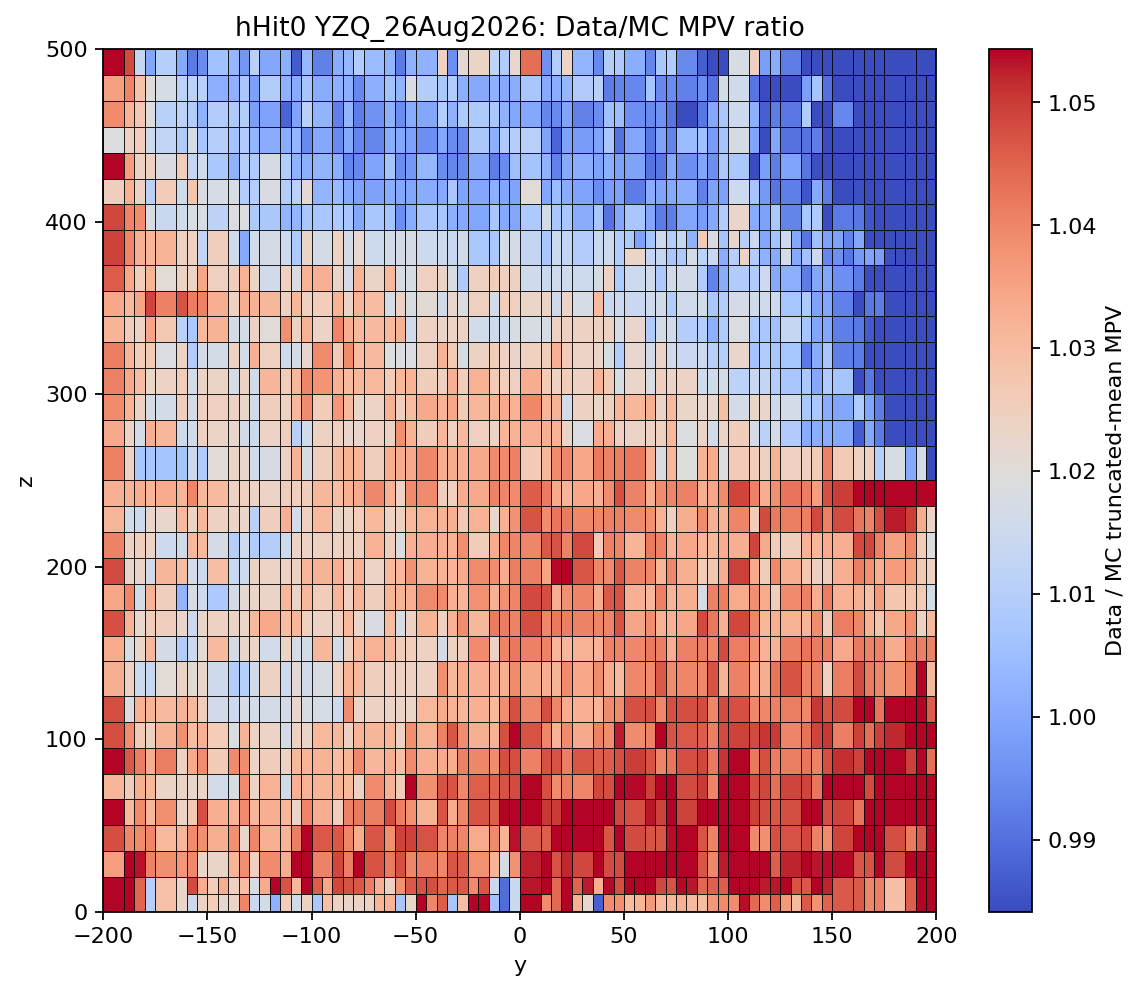
\includegraphics[width=\textwidth]{Figures/WireMod2D/ratios/YZQ_26Aug2026/hHit0_ratio_map.png}\caption{Plane 0}\end{subfigure}
\begin{subfigure}{0.31\textwidth}\centering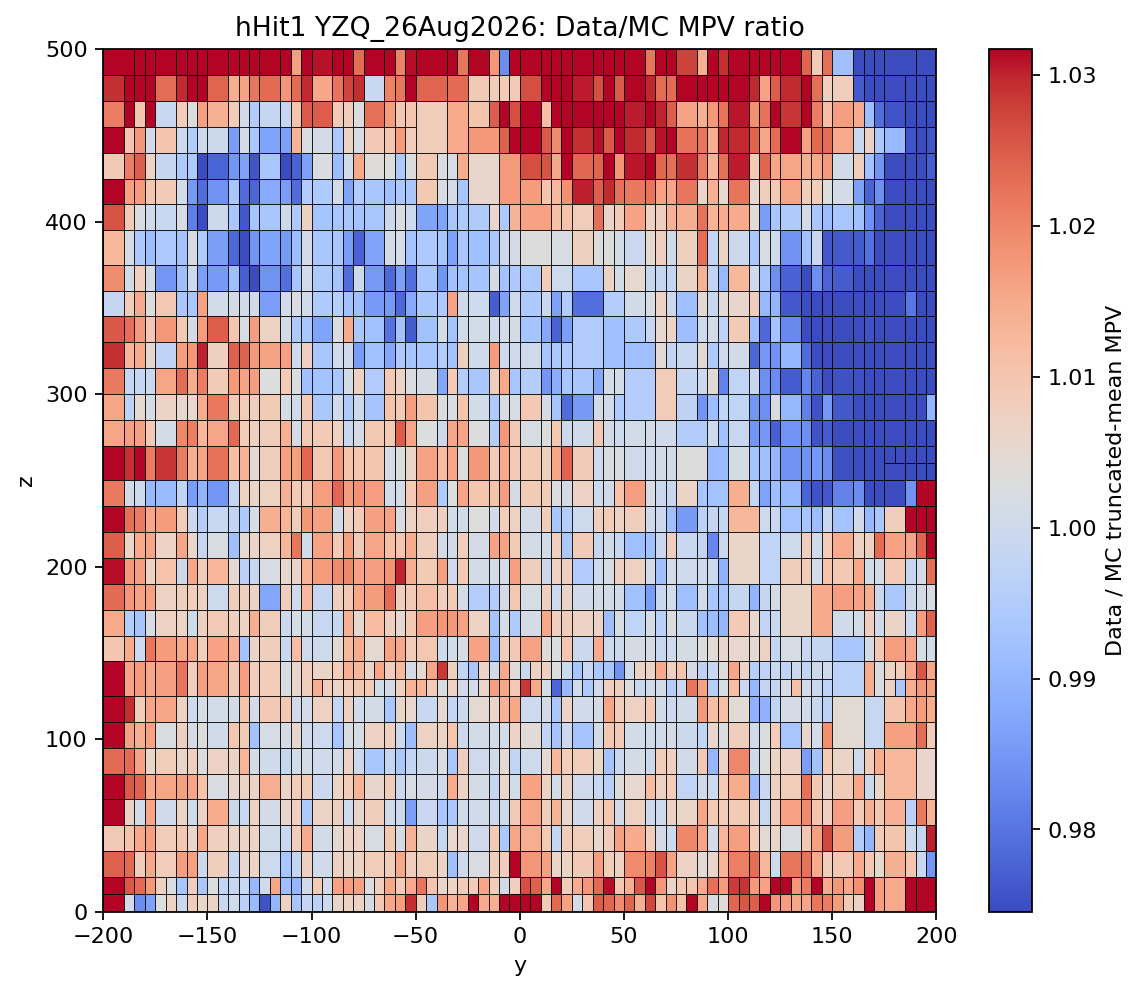
\includegraphics[width=\textwidth]{Figures/WireMod2D/ratios/YZQ_26Aug2026/hHit1_ratio_map.png}\caption{Plane 1}\end{subfigure}
\begin{subfigure}{0.31\textwidth}\centering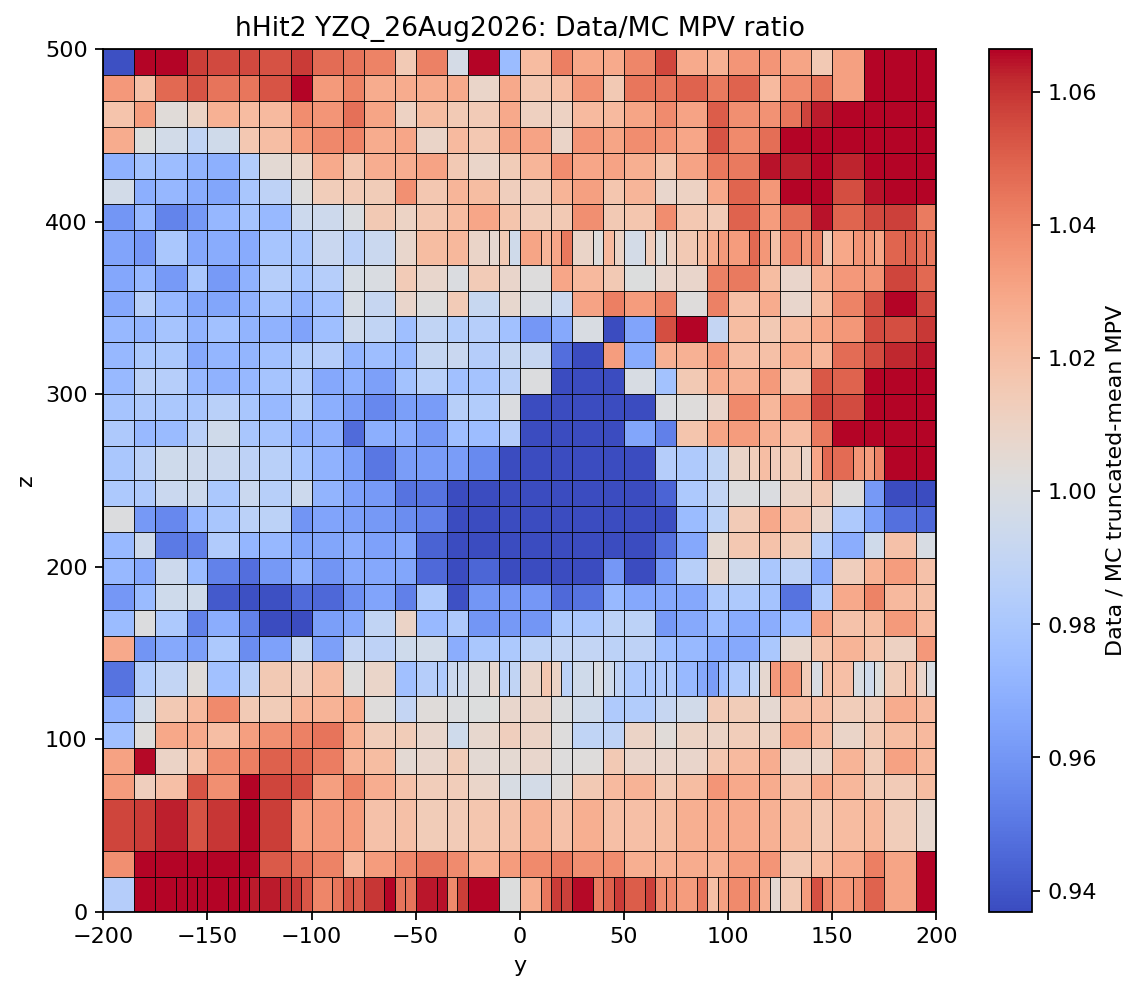
\includegraphics[width=\textwidth]{Figures/WireMod2D/ratios/YZQ_26Aug2026/hHit2_ratio_map.png}\caption{Plane 2}\end{subfigure}
\begin{subfigure}{0.31\textwidth}\centering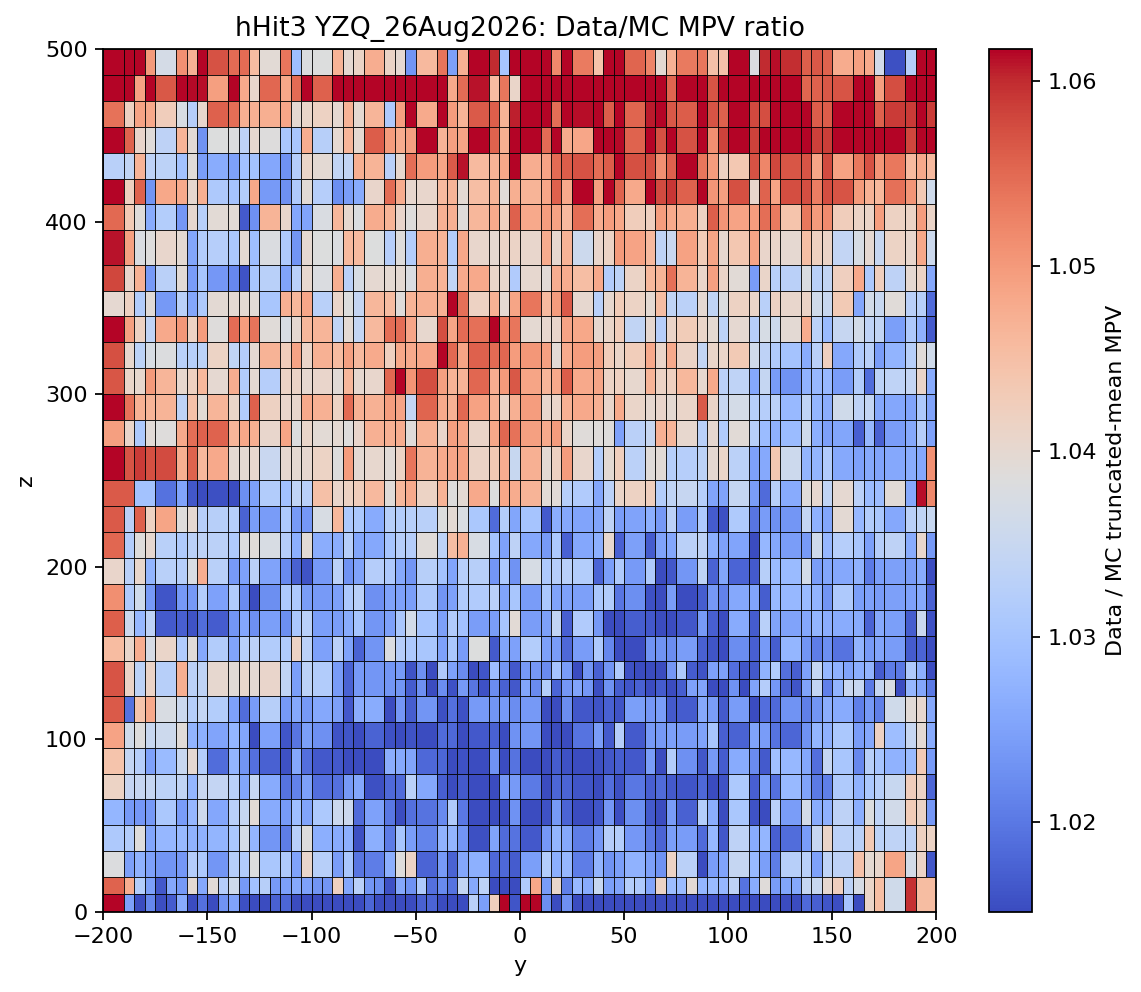
\includegraphics[width=\textwidth]{Figures/WireMod2D/ratios/YZQ_26Aug2026/hHit3_ratio_map.png}\caption{Plane 3}\end{subfigure}
\begin{subfigure}{0.31\textwidth}\centering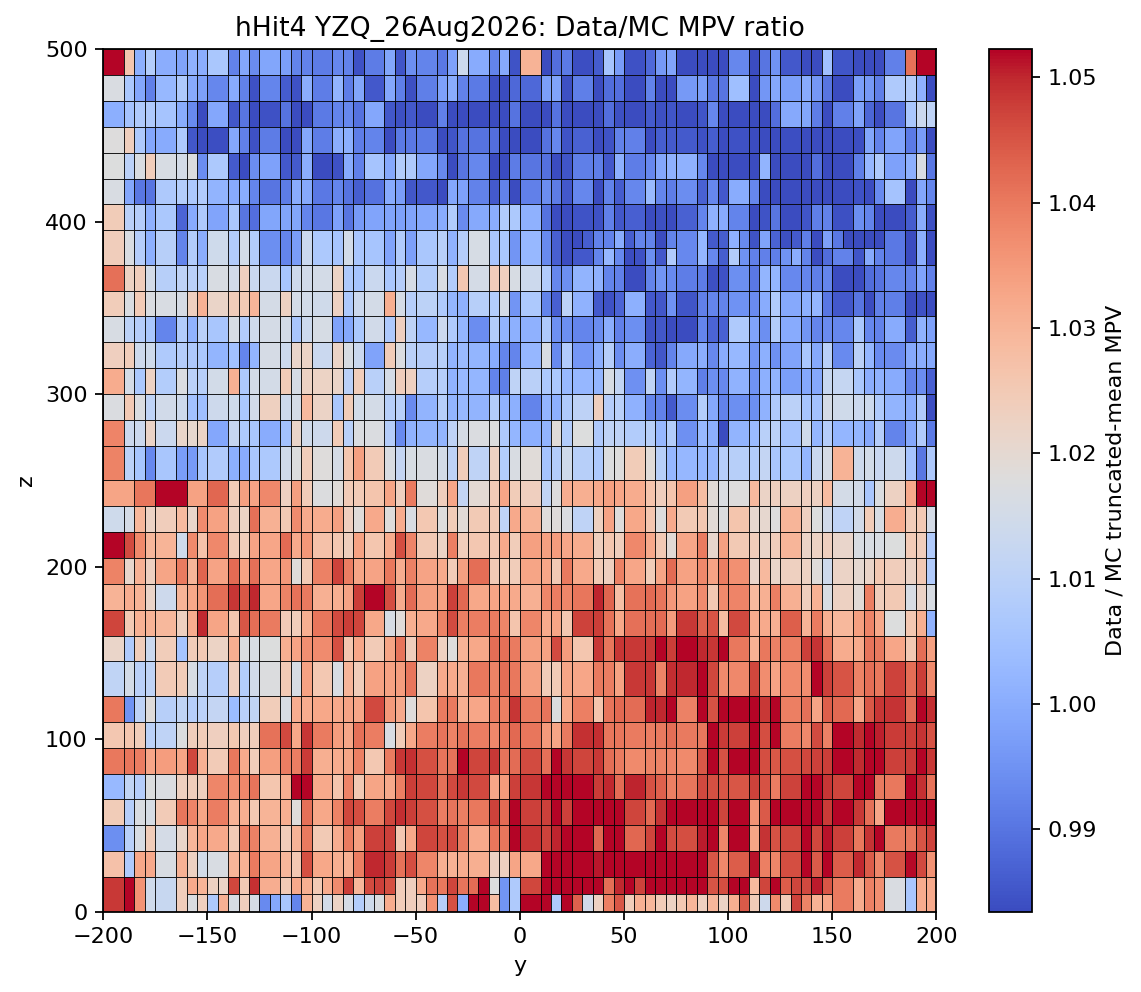
\includegraphics[width=\textwidth]{Figures/WireMod2D/ratios/YZQ_26Aug2026/hHit4_ratio_map.png}\caption{Plane 4}\end{subfigure}
\begin{subfigure}{0.31\textwidth}\centering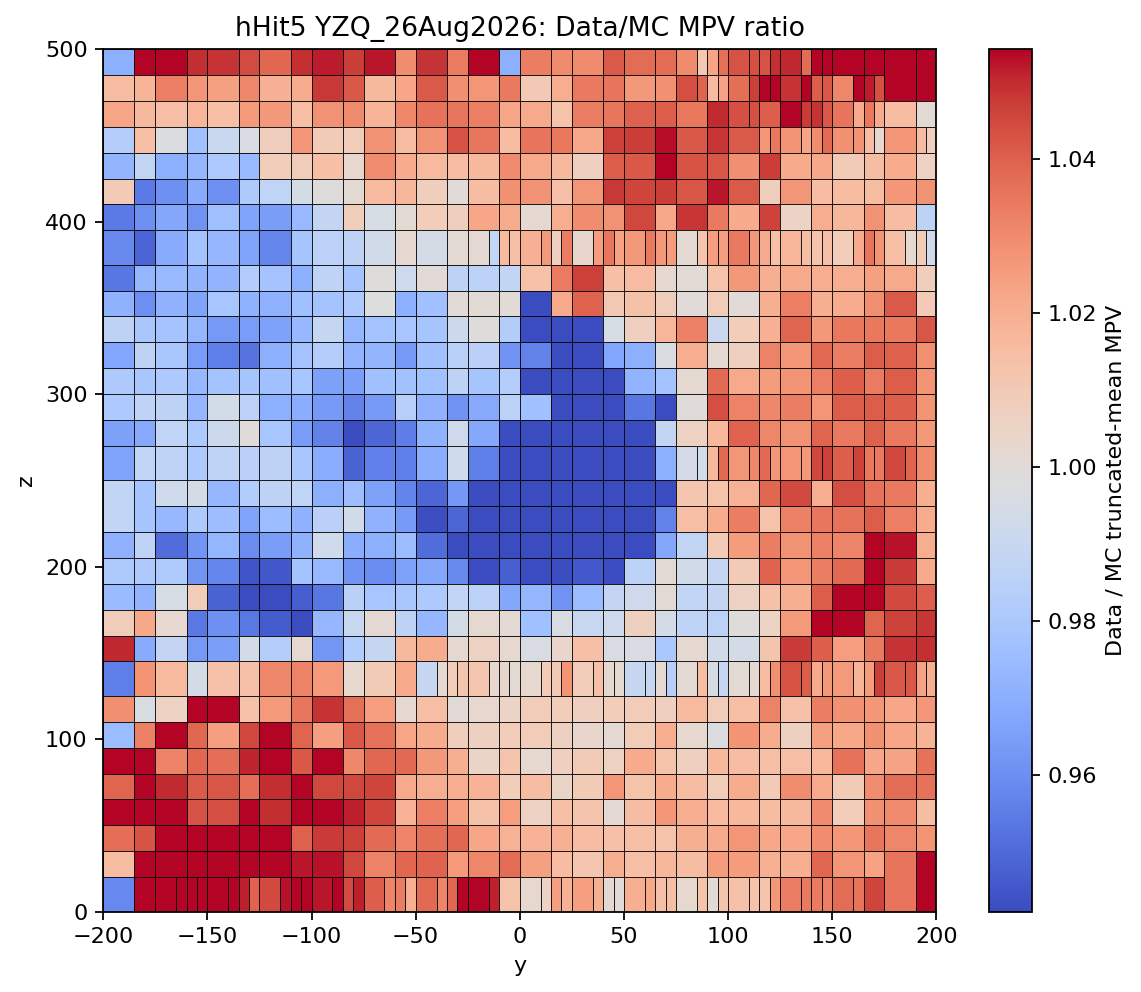
\includegraphics[width=\textwidth]{Figures/WireMod2D/ratios/YZQ_26Aug2026/hHit5_ratio_map.png}\caption{Plane 5}\end{subfigure}
\caption{\texttt{YZQ} data/MC MPV ratio maps for all planes.}
\end{figure}

\begin{figure}[H]
\centering
\begin{subfigure}{0.31\textwidth}\centering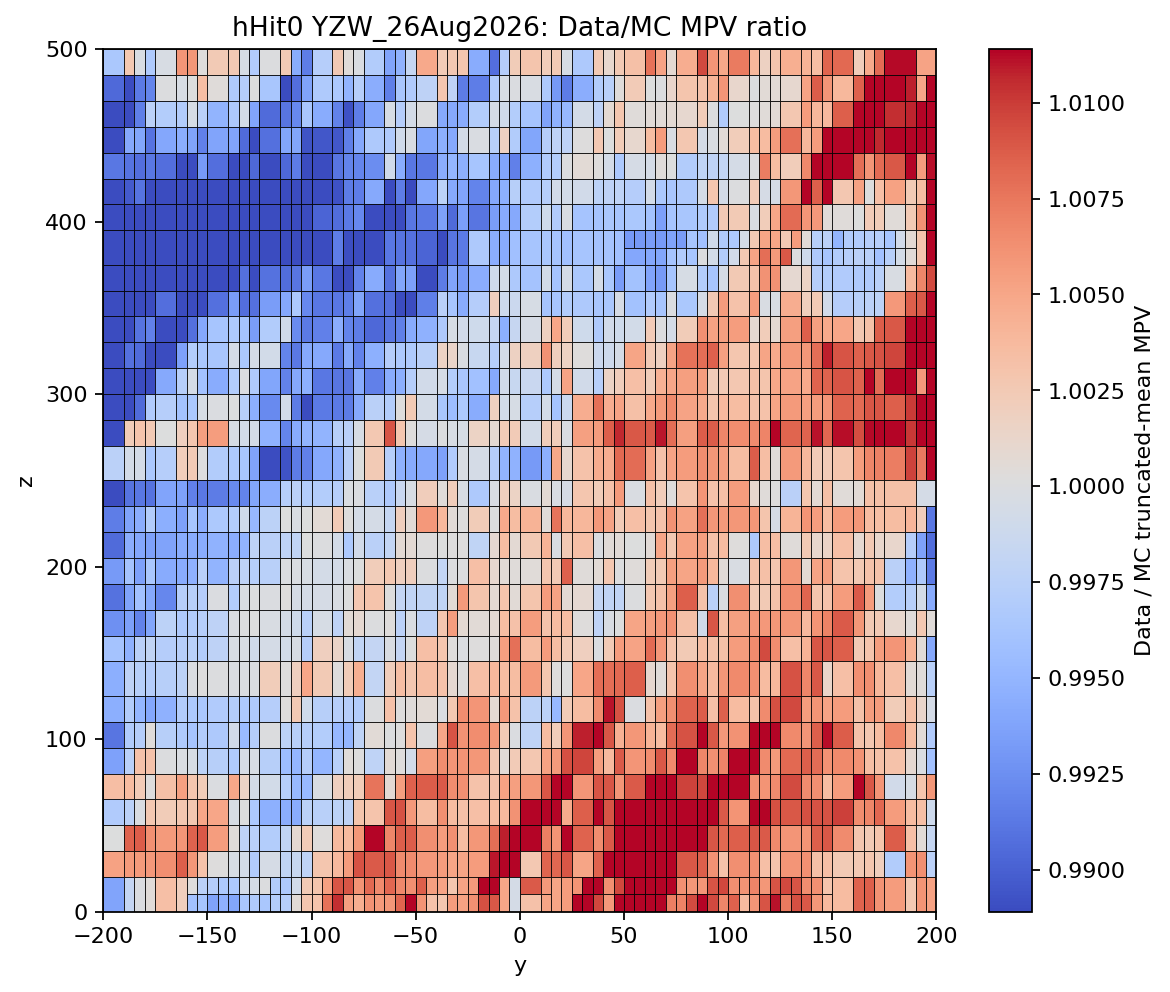
\includegraphics[width=\textwidth]{Figures/WireMod2D/ratios/YZW_26Aug2026/hHit0_ratio_map.png}\caption{Plane 0}\end{subfigure}
\begin{subfigure}{0.31\textwidth}\centering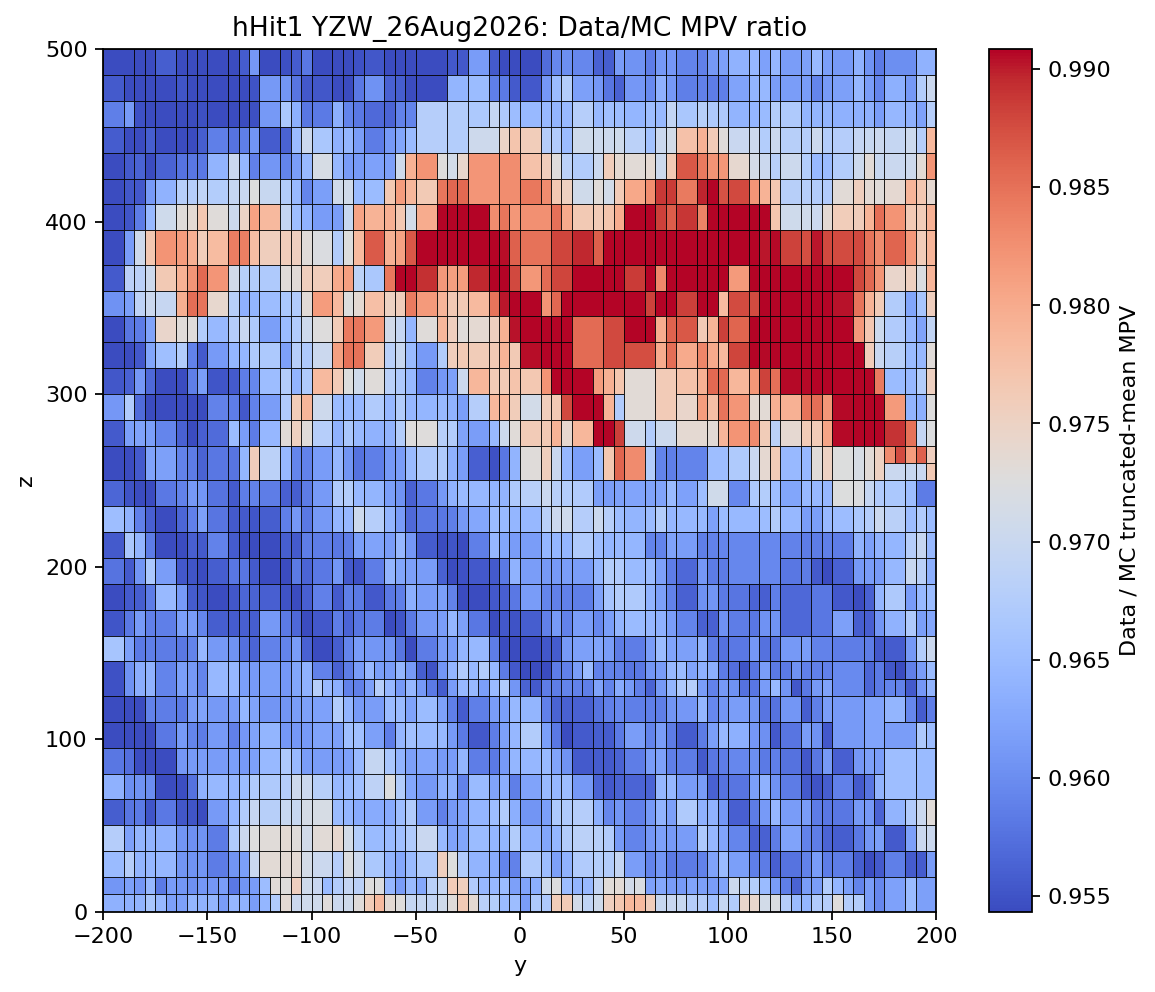
\includegraphics[width=\textwidth]{Figures/WireMod2D/ratios/YZW_26Aug2026/hHit1_ratio_map.png}\caption{Plane 1}\end{subfigure}
\begin{subfigure}{0.31\textwidth}\centering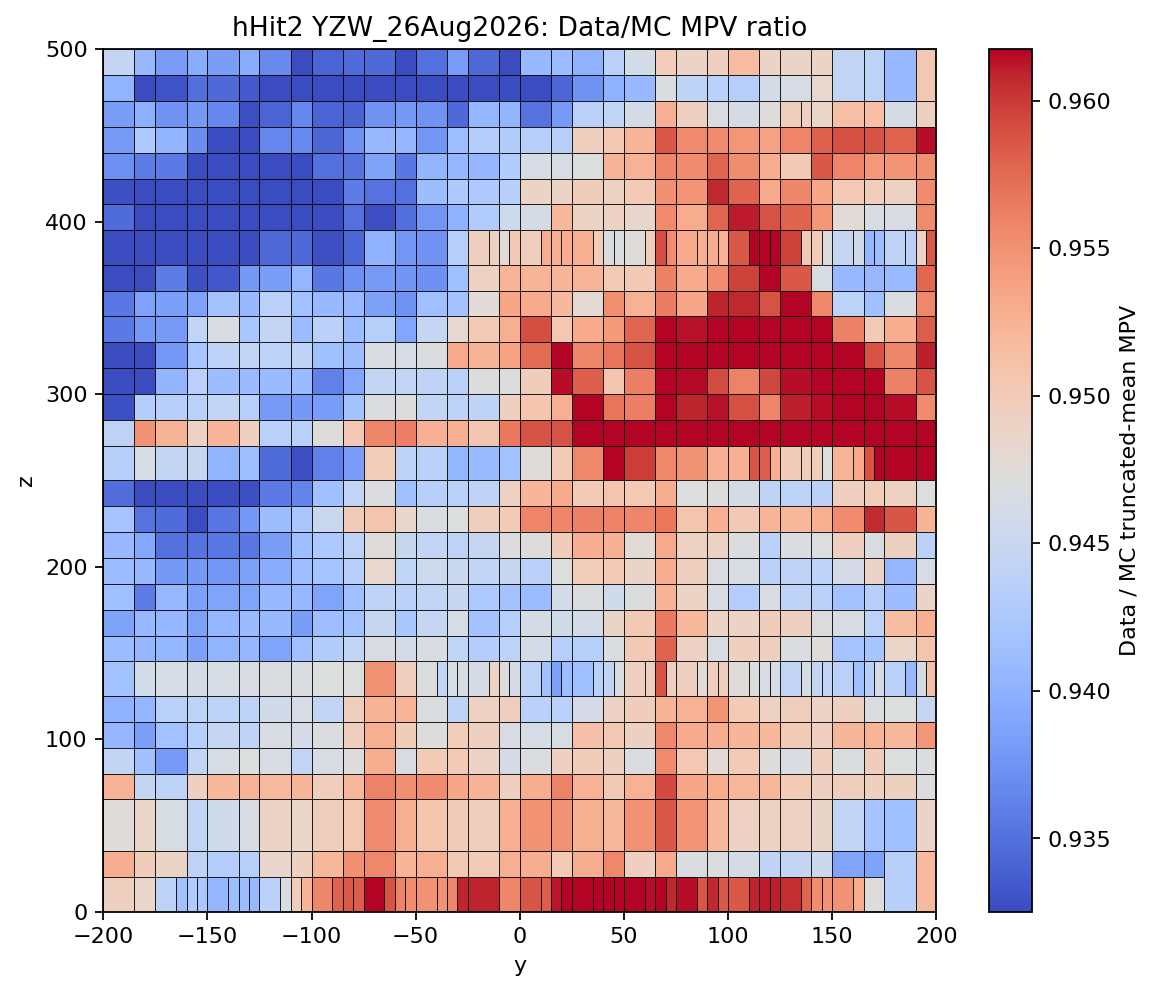
\includegraphics[width=\textwidth]{Figures/WireMod2D/ratios/YZW_26Aug2026/hHit2_ratio_map.png}\caption{Plane 2}\end{subfigure}
\begin{subfigure}{0.31\textwidth}\centering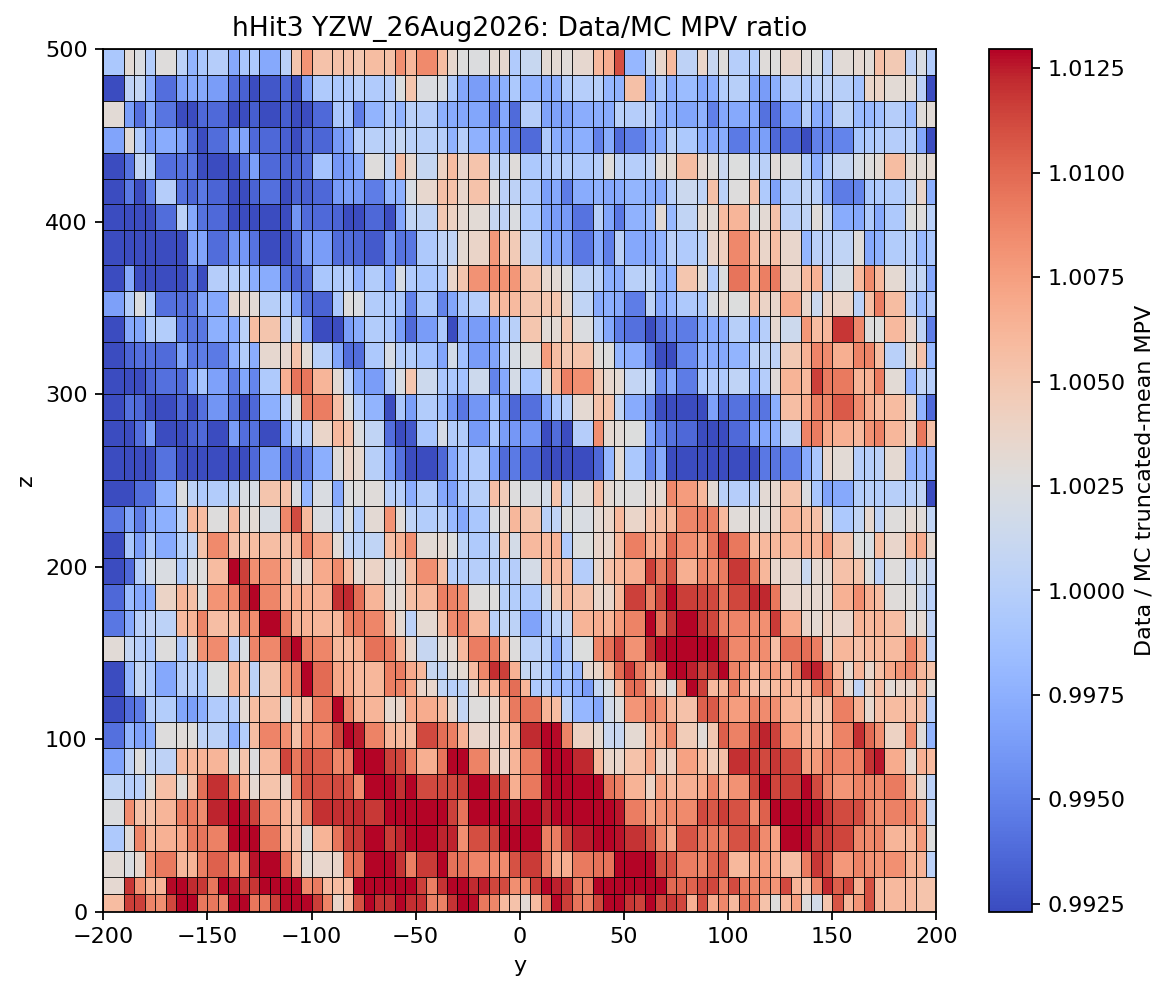
\includegraphics[width=\textwidth]{Figures/WireMod2D/ratios/YZW_26Aug2026/hHit3_ratio_map.png}\caption{Plane 3}\end{subfigure}
\begin{subfigure}{0.31\textwidth}\centering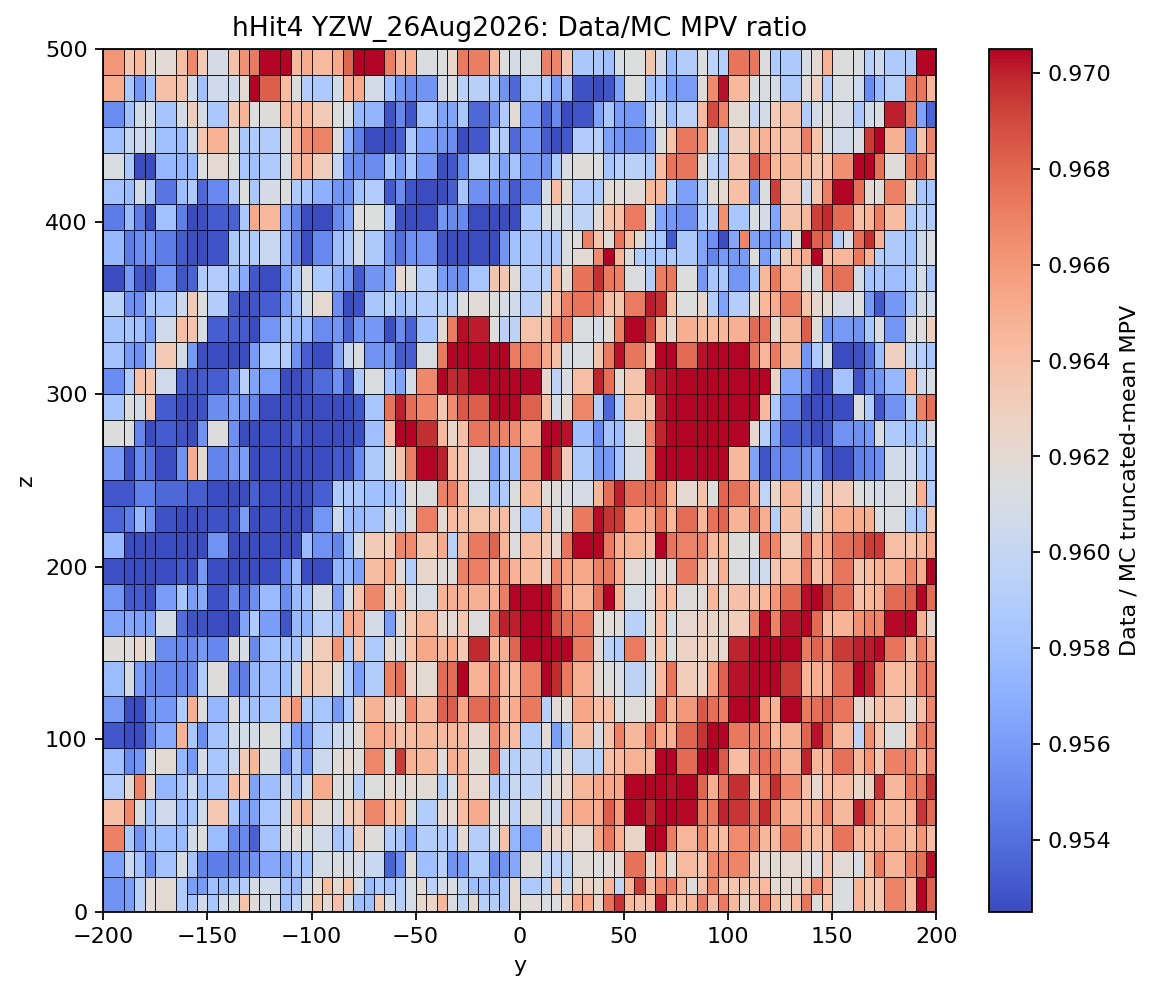
\includegraphics[width=\textwidth]{Figures/WireMod2D/ratios/YZW_26Aug2026/hHit4_ratio_map.png}\caption{Plane 4}\end{subfigure}
\begin{subfigure}{0.31\textwidth}\centering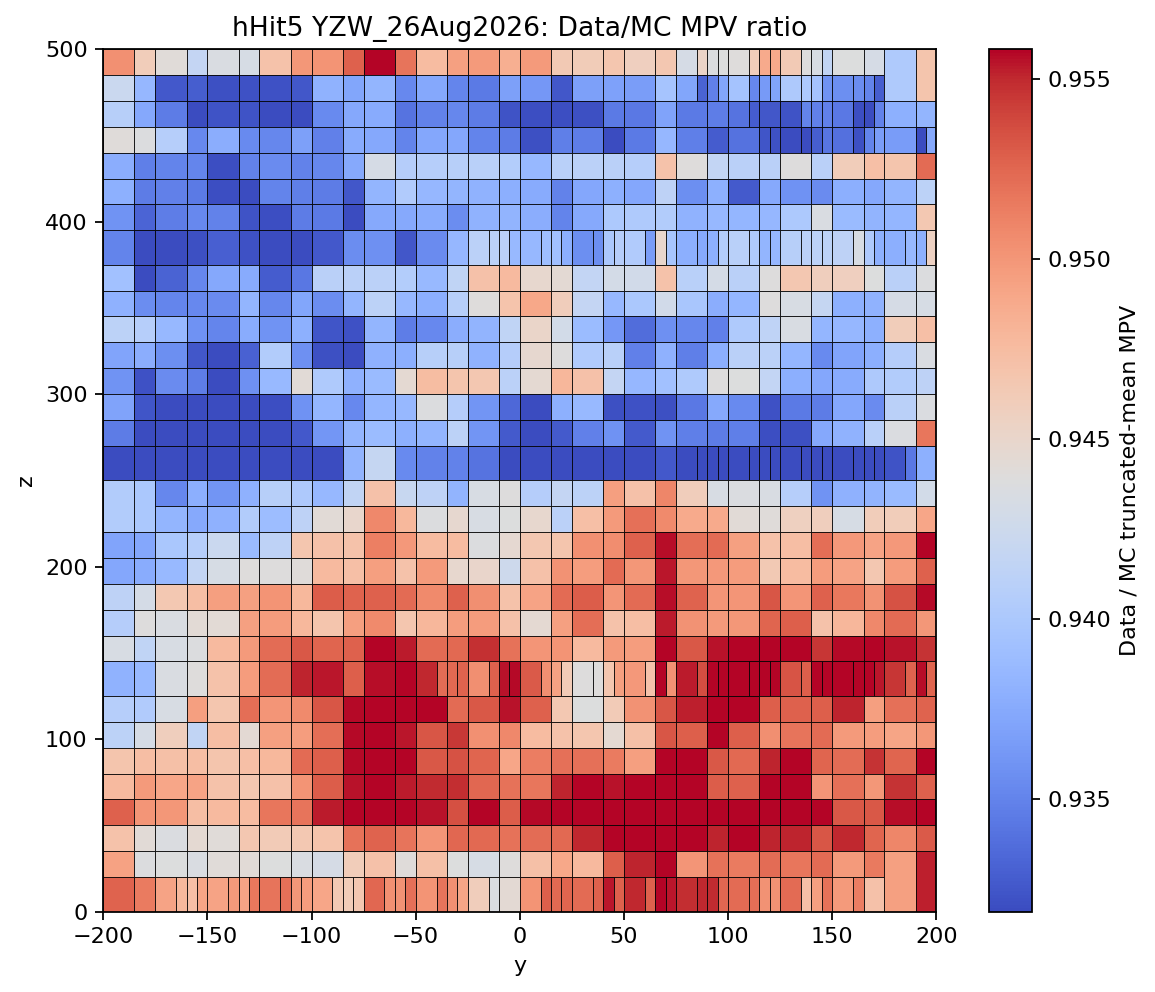
\includegraphics[width=\textwidth]{Figures/WireMod2D/ratios/YZW_26Aug2026/hHit5_ratio_map.png}\caption{Plane 5}\end{subfigure}
\caption{\texttt{YZW} data/MC MPV ratio maps for all planes.}
\end{figure}

\begin{figure}[H]
\centering
\begin{subfigure}{0.31\textwidth}\centering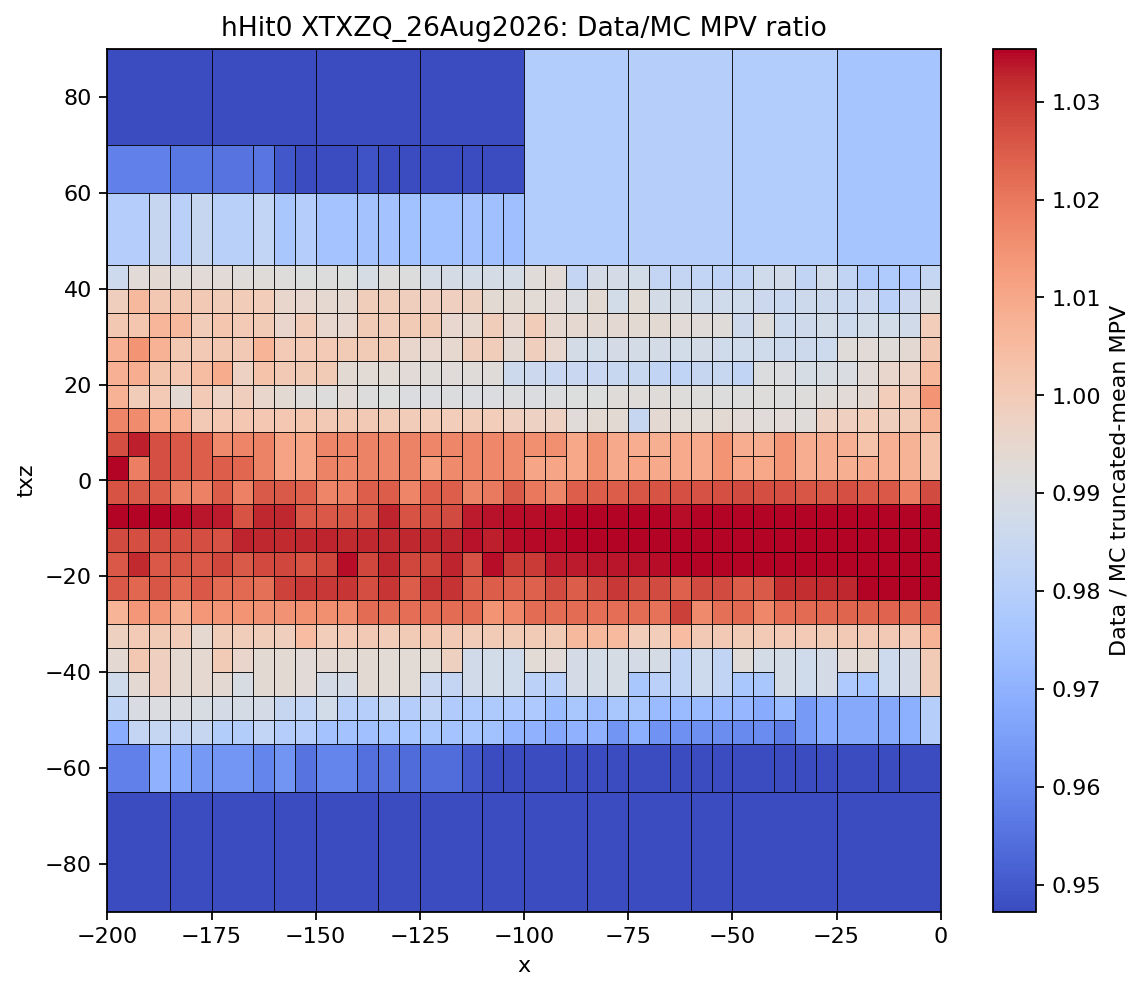
\includegraphics[width=\textwidth]{Figures/WireMod2D/ratios/XTXZQ_26Aug2026/hHit0_ratio_map.png}\caption{Plane 0}\end{subfigure}
\begin{subfigure}{0.31\textwidth}\centering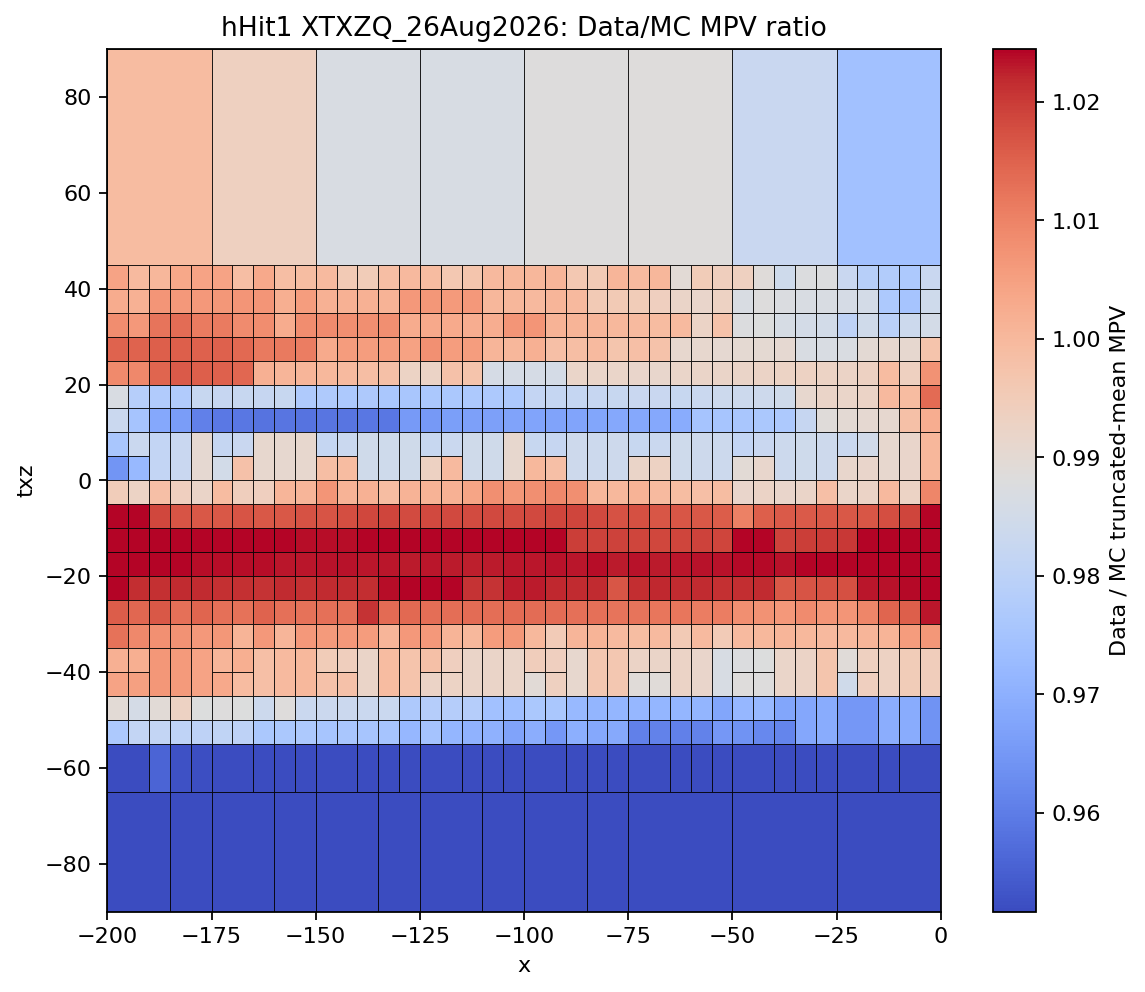
\includegraphics[width=\textwidth]{Figures/WireMod2D/ratios/XTXZQ_26Aug2026/hHit1_ratio_map.png}\caption{Plane 1}\end{subfigure}
\begin{subfigure}{0.31\textwidth}\centering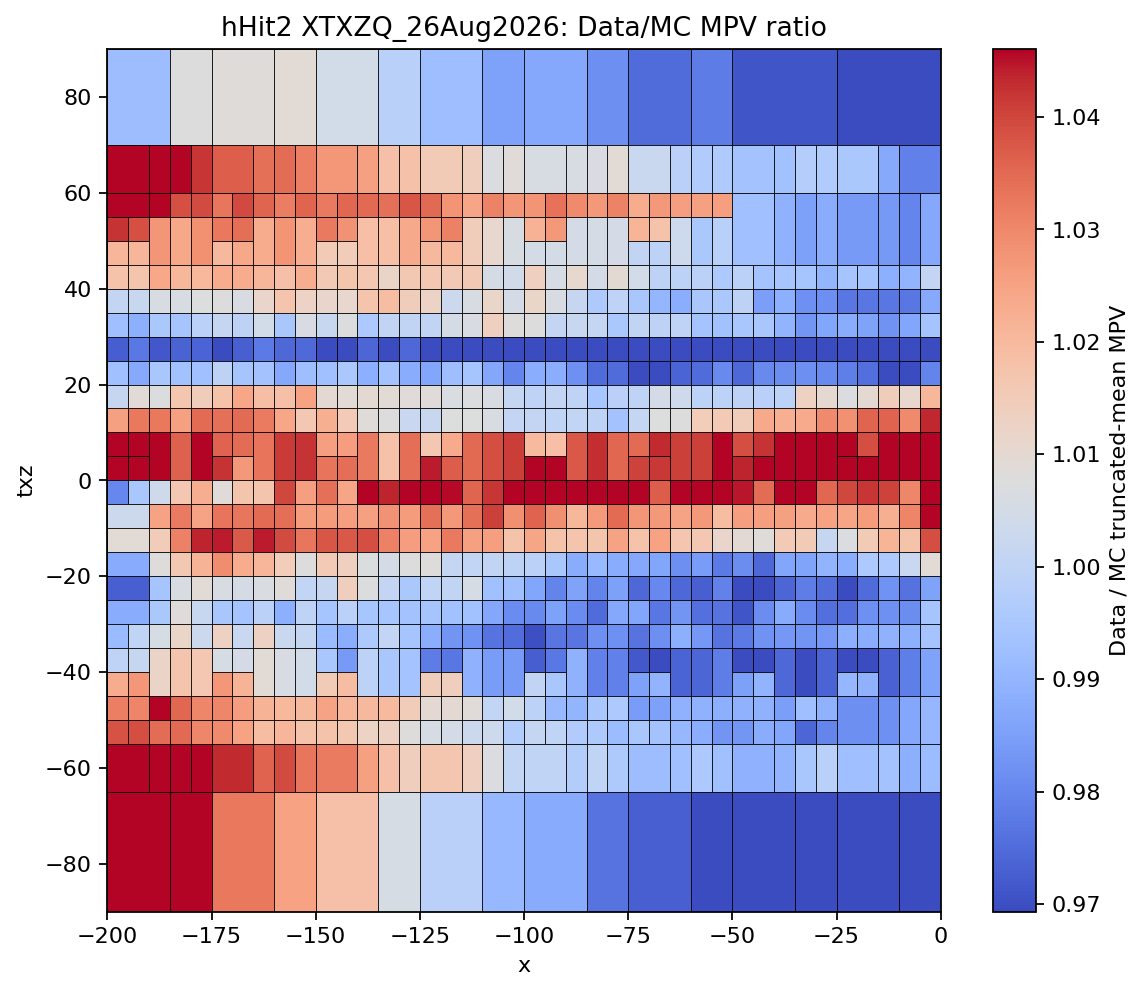
\includegraphics[width=\textwidth]{Figures/WireMod2D/ratios/XTXZQ_26Aug2026/hHit2_ratio_map.png}\caption{Plane 2}\end{subfigure}
\begin{subfigure}{0.31\textwidth}\centering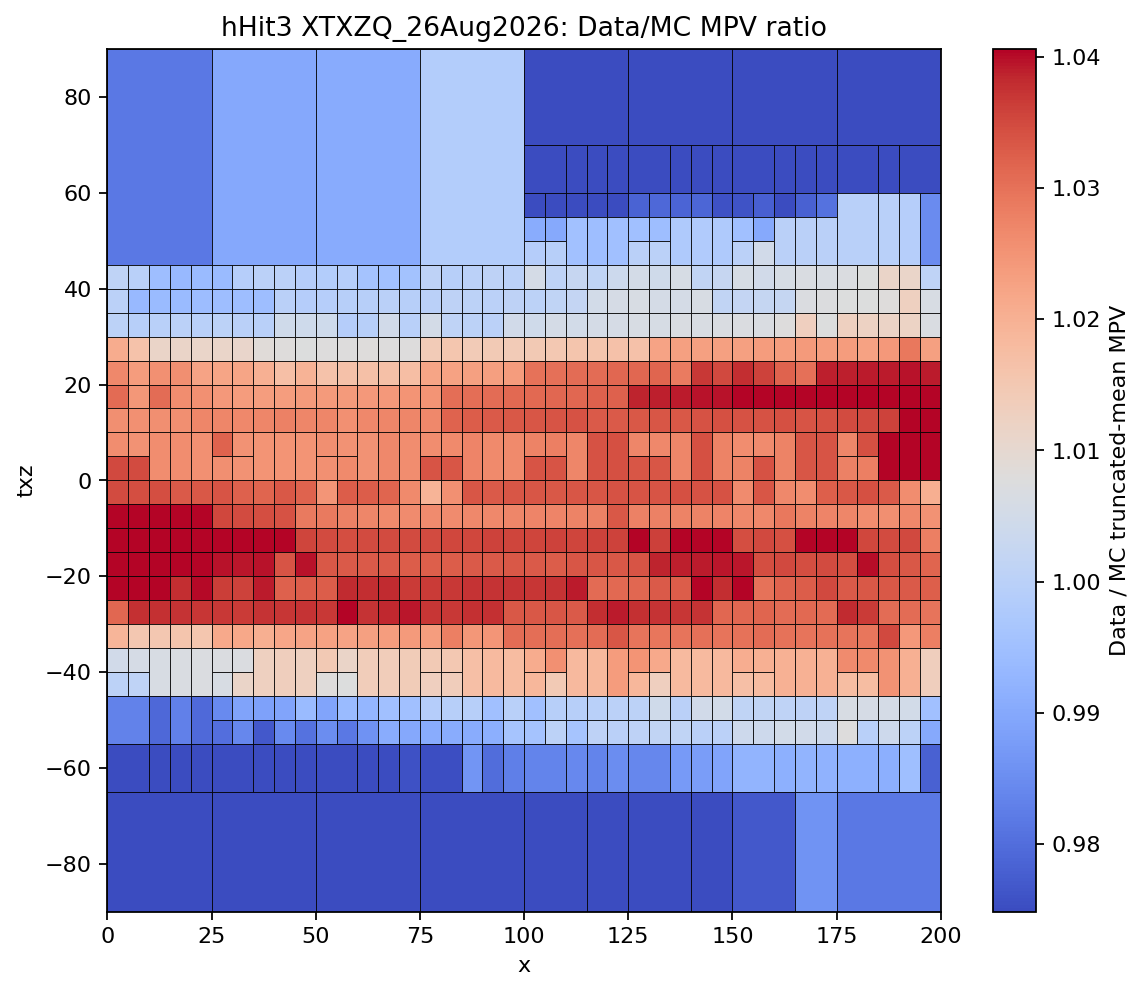
\includegraphics[width=\textwidth]{Figures/WireMod2D/ratios/XTXZQ_26Aug2026/hHit3_ratio_map.png}\caption{Plane 3}\end{subfigure}
\begin{subfigure}{0.31\textwidth}\centering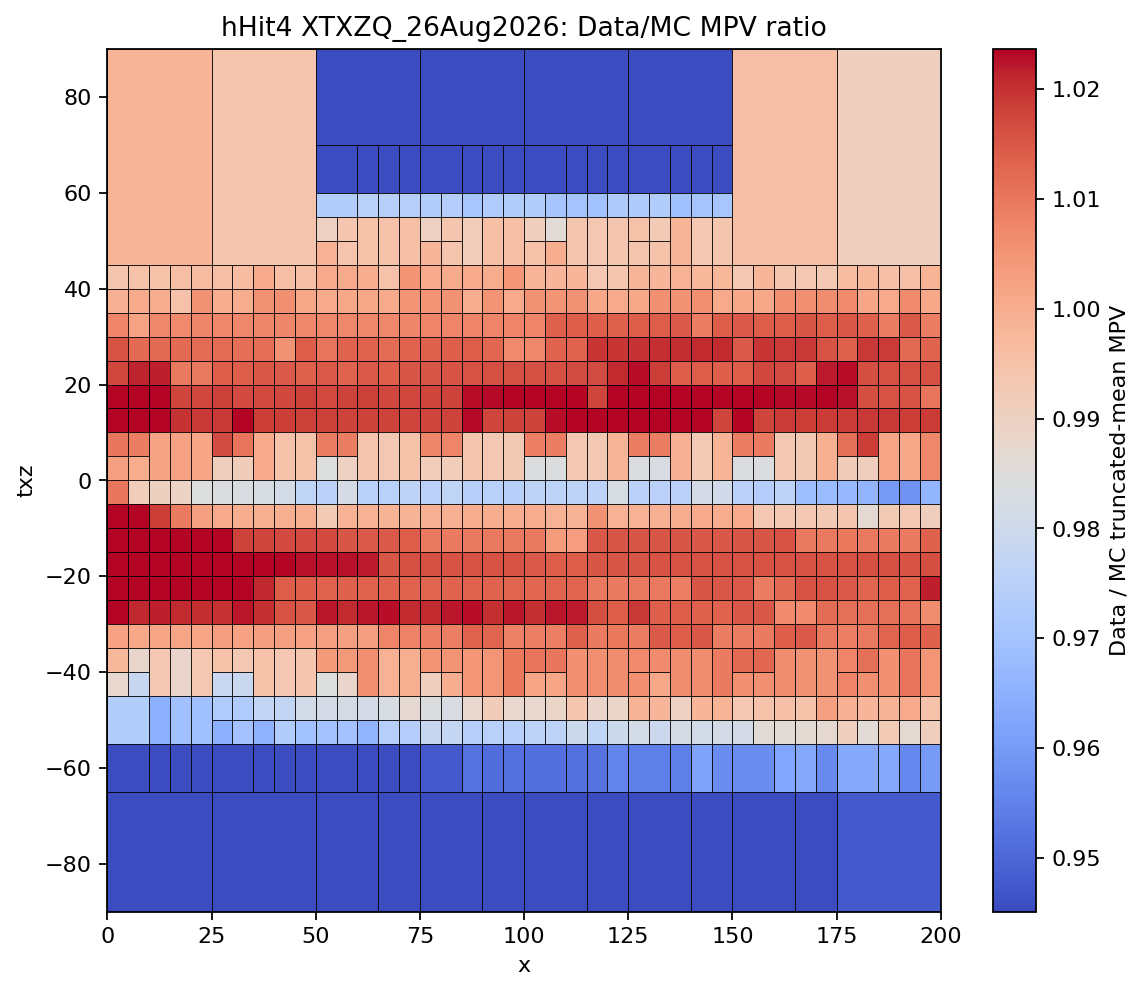
\includegraphics[width=\textwidth]{Figures/WireMod2D/ratios/XTXZQ_26Aug2026/hHit4_ratio_map.png}\caption{Plane 4}\end{subfigure}
\begin{subfigure}{0.31\textwidth}\centering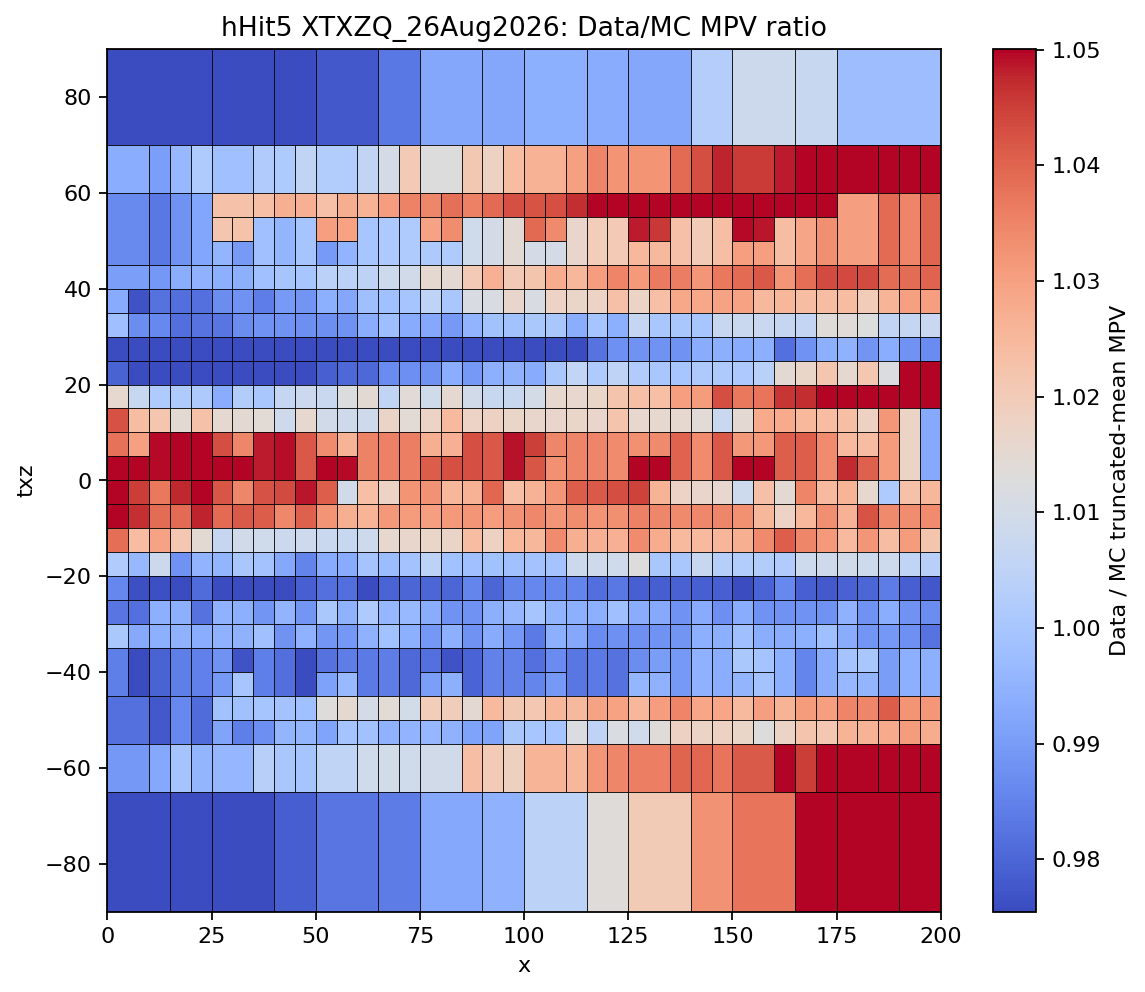
\includegraphics[width=\textwidth]{Figures/WireMod2D/ratios/XTXZQ_26Aug2026/hHit5_ratio_map.png}\caption{Plane 5}\end{subfigure}
\caption{\texttt{XTXZQ} data/MC MPV ratio maps for all planes.}
\end{figure}

\begin{figure}[H]
\centering
\begin{subfigure}{0.31\textwidth}\centering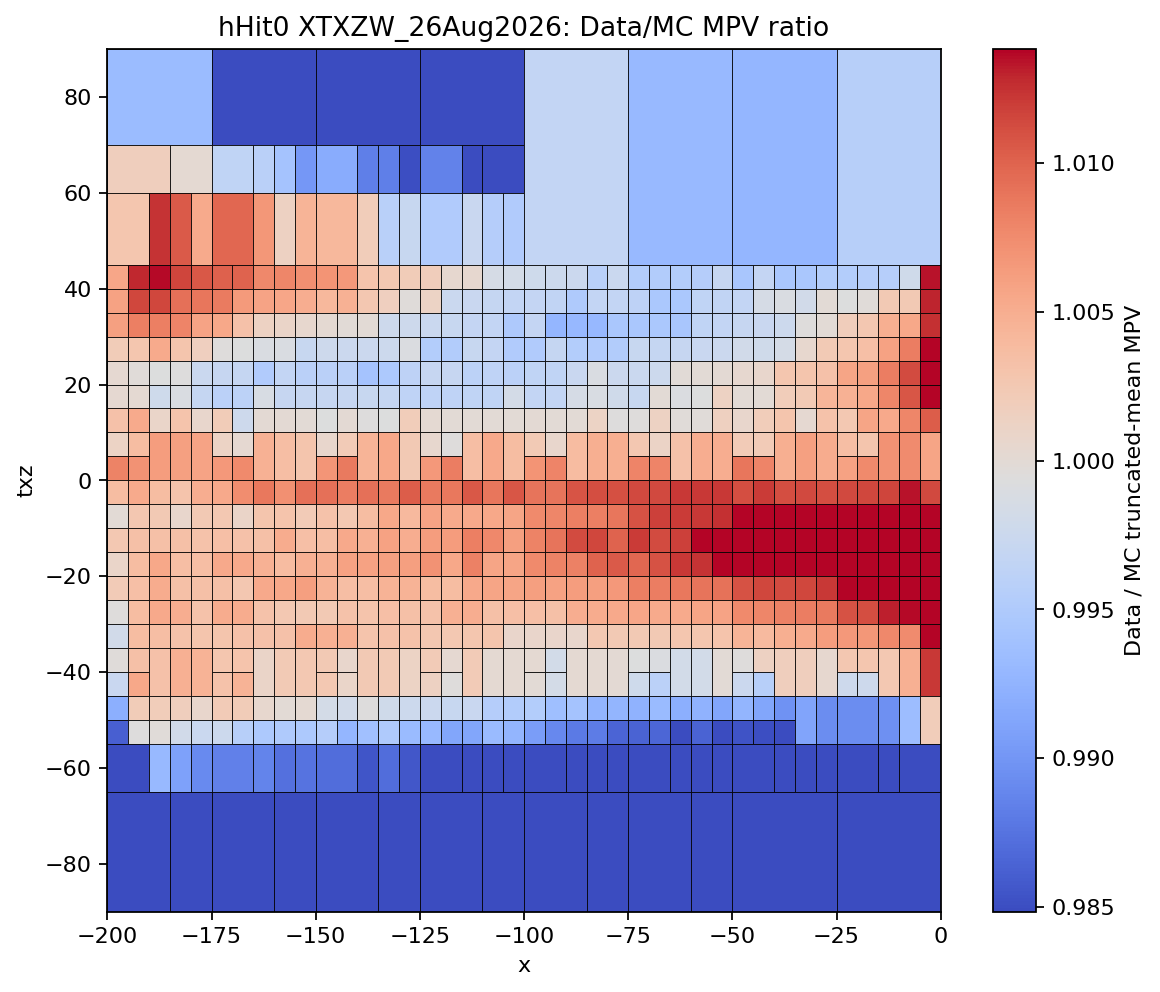
\includegraphics[width=\textwidth]{Figures/WireMod2D/ratios/XTXZW_26Aug2026/hHit0_ratio_map.png}\caption{Plane 0}\end{subfigure}
\begin{subfigure}{0.31\textwidth}\centering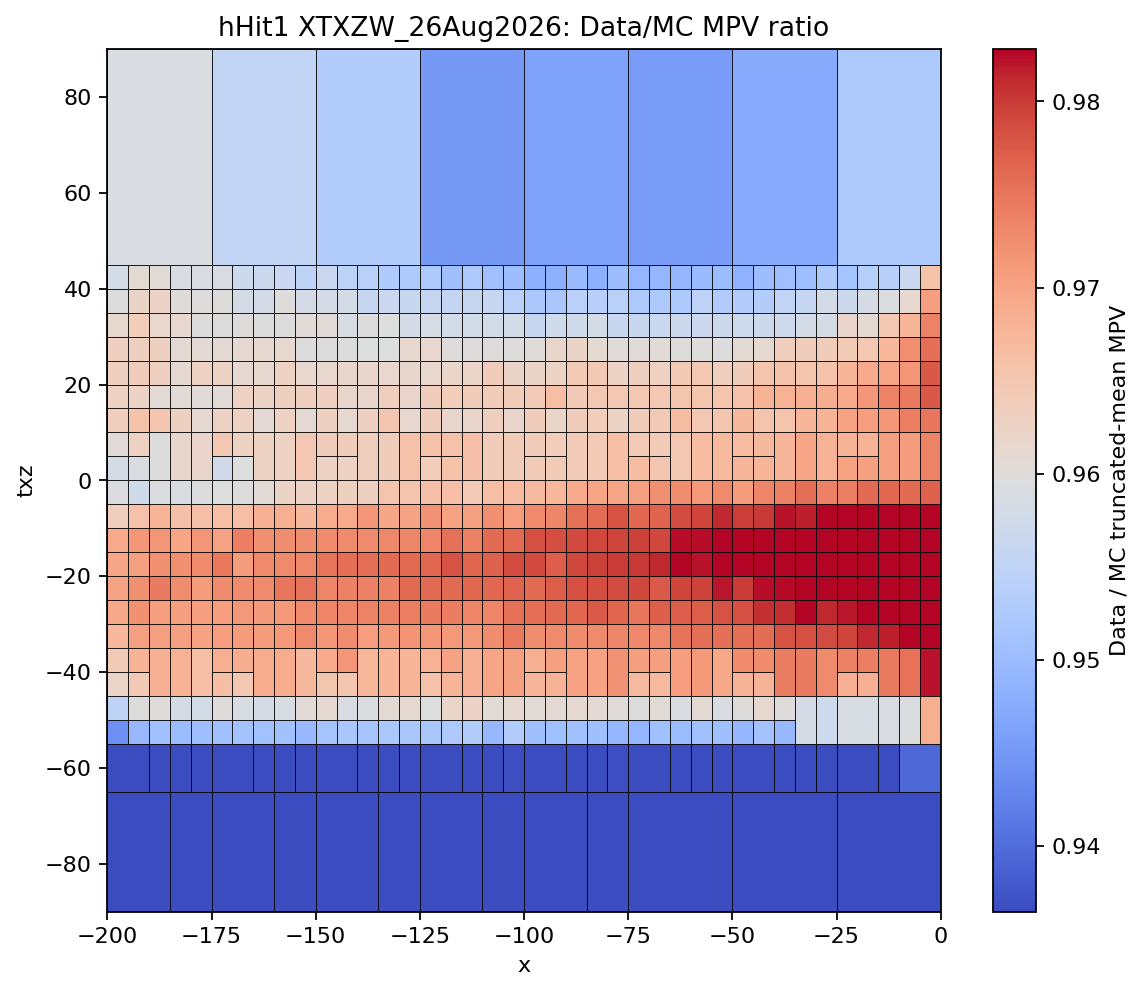
\includegraphics[width=\textwidth]{Figures/WireMod2D/ratios/XTXZW_26Aug2026/hHit1_ratio_map.png}\caption{Plane 1}\end{subfigure}
\begin{subfigure}{0.31\textwidth}\centering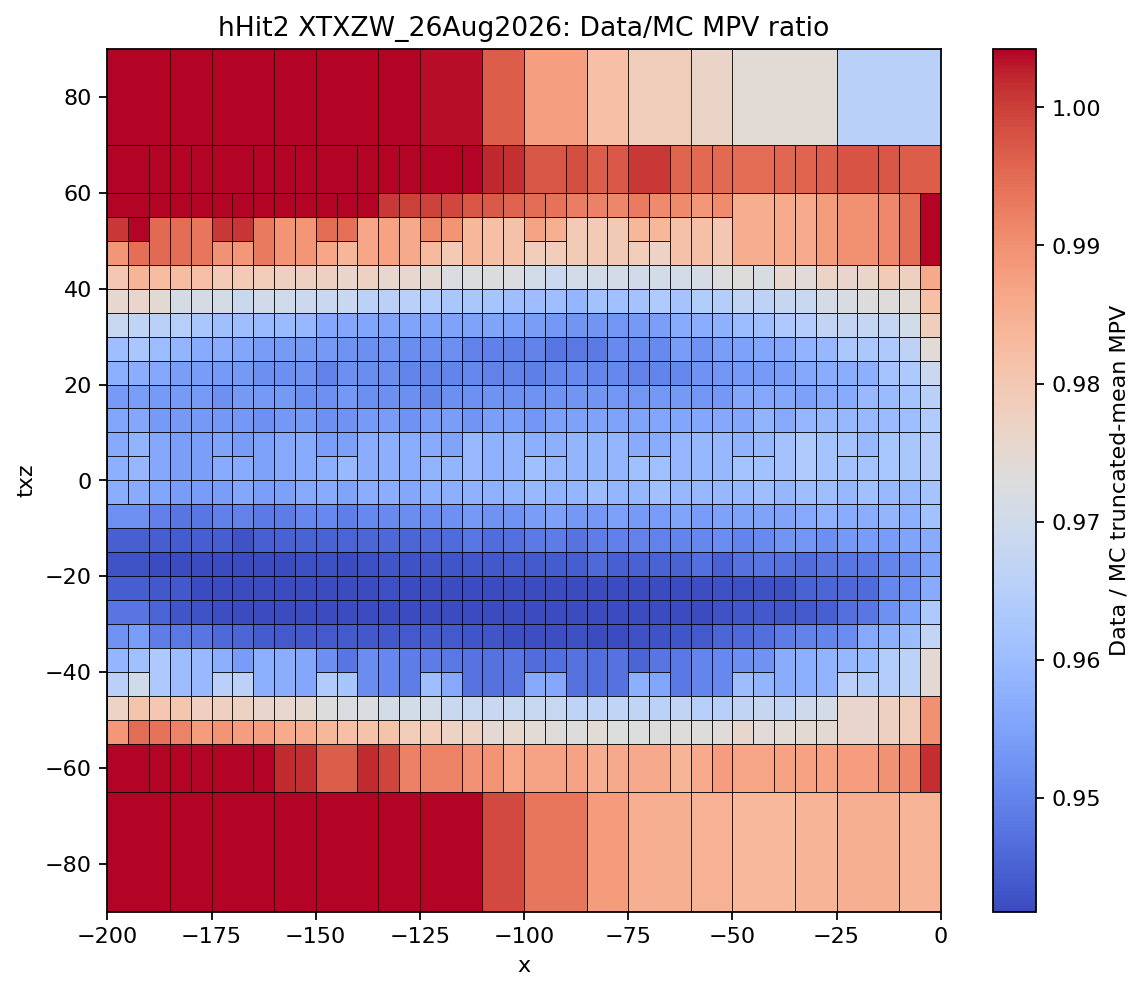
\includegraphics[width=\textwidth]{Figures/WireMod2D/ratios/XTXZW_26Aug2026/hHit2_ratio_map.png}\caption{Plane 2}\end{subfigure}
\begin{subfigure}{0.31\textwidth}\centering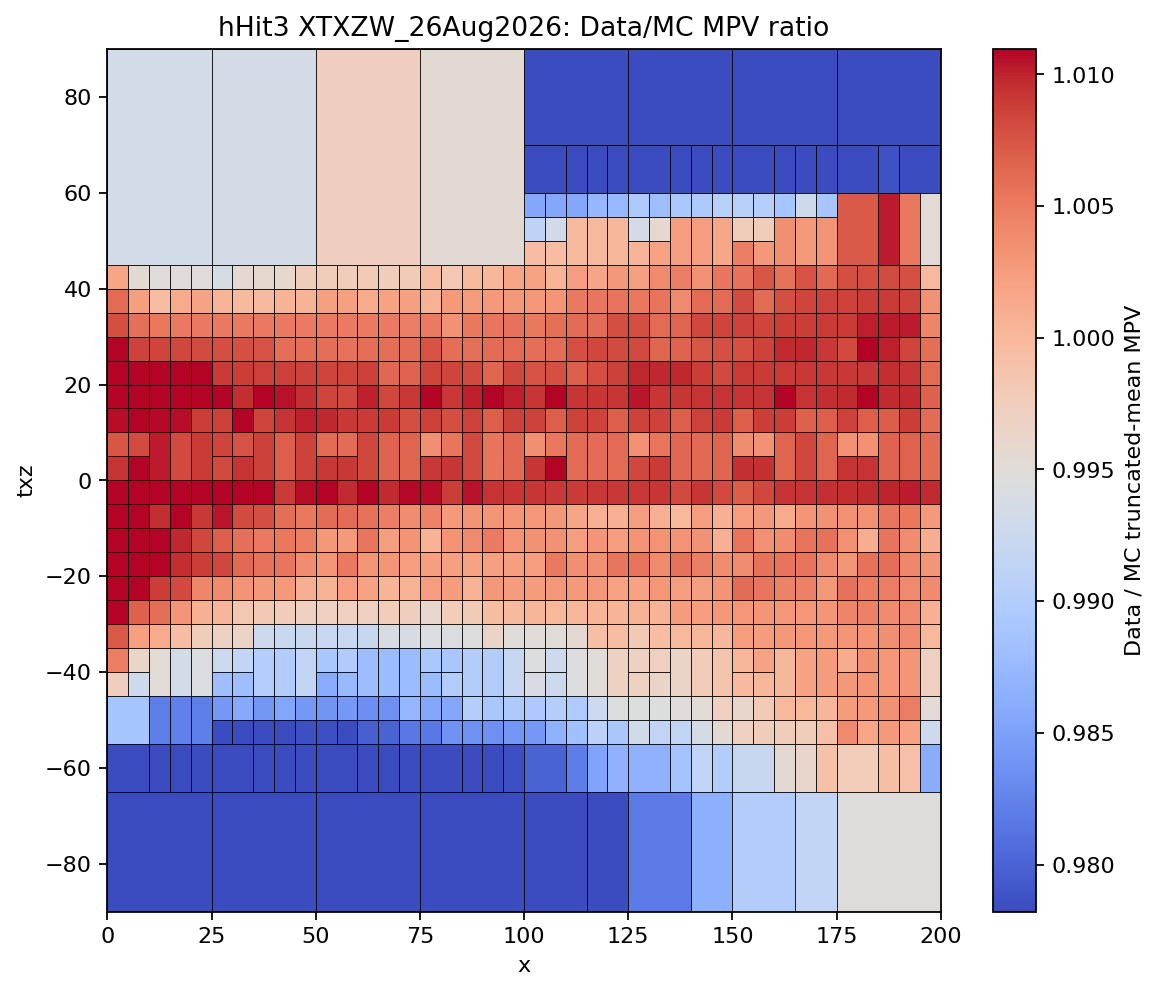
\includegraphics[width=\textwidth]{Figures/WireMod2D/ratios/XTXZW_26Aug2026/hHit3_ratio_map.png}\caption{Plane 3}\end{subfigure}
\begin{subfigure}{0.31\textwidth}\centering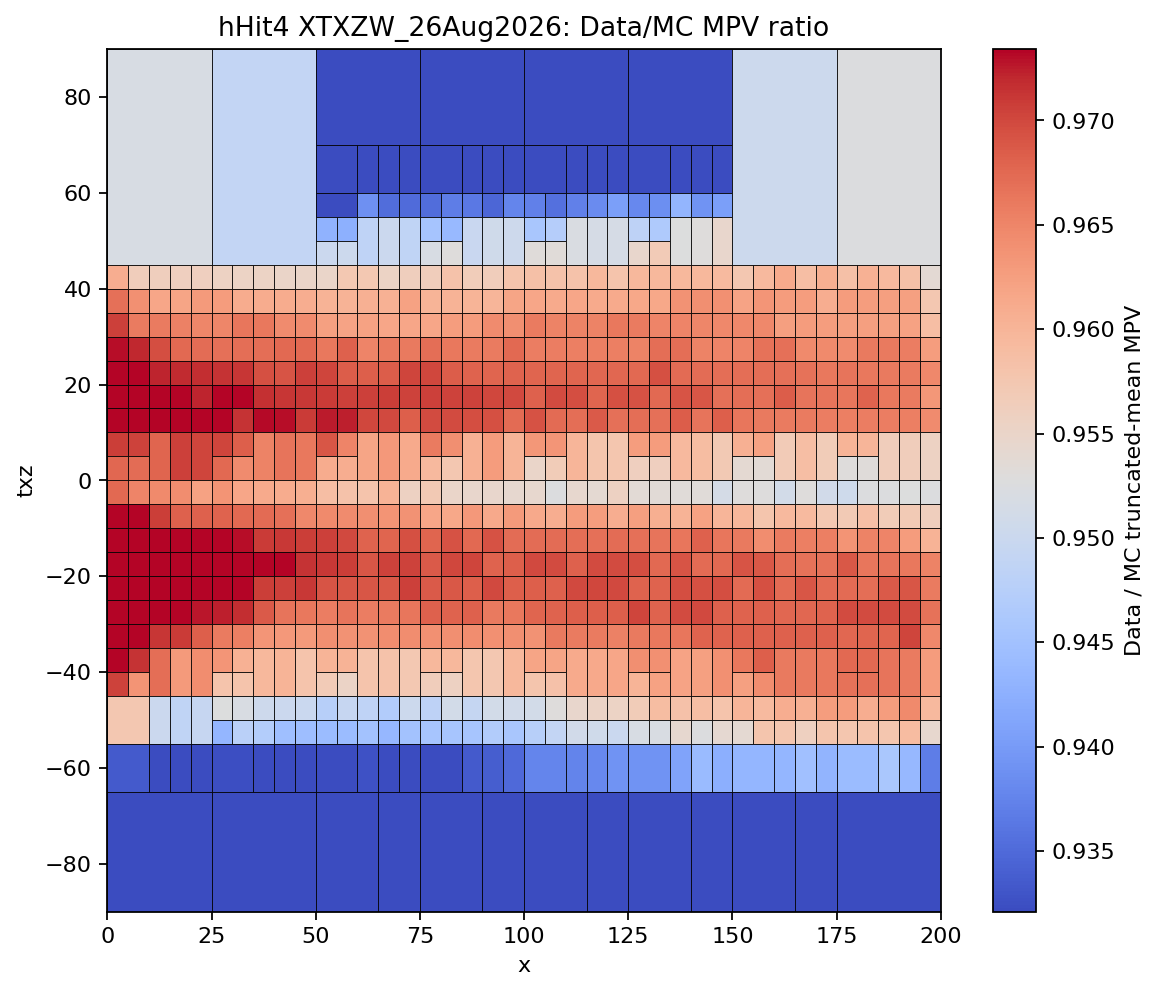
\includegraphics[width=\textwidth]{Figures/WireMod2D/ratios/XTXZW_26Aug2026/hHit4_ratio_map.png}\caption{Plane 4}\end{subfigure}
\begin{subfigure}{0.31\textwidth}\centering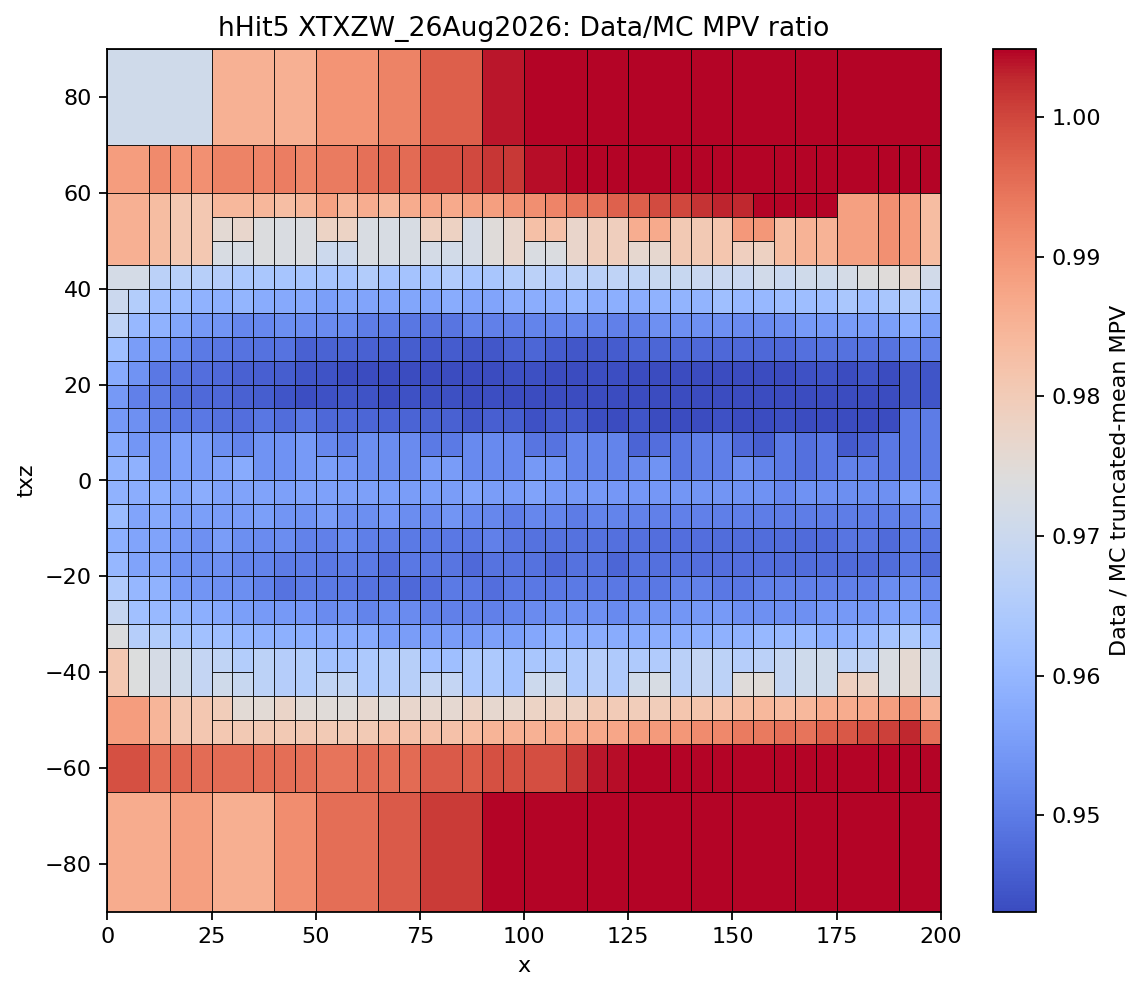
\includegraphics[width=\textwidth]{Figures/WireMod2D/ratios/XTXZW_26Aug2026/hHit5_ratio_map.png}\caption{Plane 5}\end{subfigure}
\caption{\texttt{XTXZW} data/MC MPV ratio maps for all planes.}
\end{figure}


\newpage







\end{appendices}


\end{document}
